\documentclass[hyperref={pdfpagelabels=true}]{beamer}
%\usepackage{etex} % Math fonts misbehave
\usepackage{lmodern} 
%\usefonttheme{structurebold}

\usepackage{gauss}
\usepackage{amsmath}
\usepackage{amsfonts}
\usepackage{lipsum}
\usepackage{graphicx}
\usepackage{subfigure}
\usepackage{setspace}
\usepackage{amssymb}
\usepackage{multirow}
\usepackage{xcolor}
\usepackage{ragged2e}
\usepackage{mathrsfs}
\usepackage{bbold}
\usepackage{tikz}
\usetikzlibrary{patterns}
\usetikzlibrary{calc}
\usetikzlibrary{matrix}
\usetikzlibrary{positioning}
\tikzset{>=stealth}
%\usepackage[all]{xy}  


\setbeamertemplate{footline}[frame number]
\setbeamercolor{normal text}{bg=white!10}
\setbeamertemplate{theorems}[numbered]

\newcommand{\C}{\mathbb{C}} \newcommand{\F}{\mathbb{F}} \newcommand{\R}{\mathbb{R}} \newcommand{\Q}{\mathbb{Q}}
\newcommand{\N}{\mathbb{N}}
\newcommand{\Z}{\mathbb{Z}}
\renewcommand{\L}{\mathcal{L}}
\newcommand{\Mat}{\text{Mat}}

\newcommand{\HRule}{\rule{\linewidth}{0.5mm}}
\newcommand{\U}{\mathrm}
\newcommand{\celsius}{\ensuremath{^{\circ}\mathrm{C}}}
\newcommand{\myseries}[2]{#1_1,\ldots,#1_{#2}}
\newcommand{\highlightr}[1]{\textcolor[rgb]{1,0.3,0.2}{\emph{\textbf{#1}}}}
\newcommand{\highlightg}[1]{\textcolor[rgb]{0.1,0.5,0.3}{\emph{\textbf{#1}}}}
\newcommand{\structb}[1]{\textcolor[rgb]{0.2,0.2,0.7}{#1}}
\newcommand{\bemph}[1]{\emph{\textbf{#1}}}
\newcommand{\tabincell}[2]{\begin{tabular}{@{}#1@{}}#2\end{tabular}}
\newcommand{\<}{\langle}
\renewcommand{\>}{\rangle}

\renewcommand\arraystretch{1.8}
\newenvironment{shrinkeq}[1]%缩短公式之间的距离
{ \bgroup
  \addtolength\abovedisplayshortskip{#1}
  \addtolength\abovedisplayskip{#1}
  \addtolength\belowdisplayshortskip{#1}
  \addtolength\belowdisplayskip{#1}}
{\egroup\ignorespacesafterend}


\title{Honors Mathematics \\Introduction to Linear Algebra}
\author{Yao Shaoxiong} 
\date{\today} 
\institute[UM-JI]{UM-SJTU Joint Institute}


\AtBeginSubsection[]{
\begin{frame}
\tableofcontents[sectionstyle=show/shaded,subsectionstyle=show/shaded]
\end{frame}
}

\begin{document}



\begin{frame}
\titlepage
\end{frame} 


\begin{frame}
\frametitle{Table of contents}
\tableofcontents
\end{frame} 

\section{Introduction to Linear Algebra}
\subsection{Systems of Linear Equations}
\begin{frame}{Linear System}
    \begin{block}{}
        For a vector space $V$ together with a field $\F$.\\
        A \highlightg{linear system} of $m$ (algebraic) equations in $n$ unknowns $x_1,...,x_n \in V$ is a set of equations
        \begin{equation}
        \begin{aligned}
            a_{11}x_1+a_{12}x_2+...+a_{1n}x_n &= b_1 \\
            a_{21}x_1+a_{22}x_2+...+a_{2n}x_n &= b_2 \\ 
            &\vdots \\
            a_{m1}x_1+a_{m2}x_2+...+a_{mn}x_n &= b_m \\
        \end{aligned}
        \label{(1)}
        \end{equation}
        where $b_{1},...,b_{m} \in V$ and $a_{ij} \in \F$, $i = 1,...,m, j = 1,...,n.$

        

        \structb{Comment:} Note that vector spaces are not limited to $\R^{n}$ and fields are not limited to $\R$ and $\C$.
    \end{block}
\end{frame}
\begin{frame}{Linear System}
    \begin{block}{}
        \begin{itemize}
            \item If $b_{1} = b_{2} = ... = b_{m} = 0$, then Eq. \ref{(1)} is called a \highlightg{homogeneous system}. Otherwise, it is called an \highlightg{inhomogeneous system.}
            \item If $m > n$ we say that the system is \highlightg{underdetermined}, if $m > n$ it is called \highlightg{overdetermined}.
            \item A \highlightg{solution} of a linear system \ref{(1)} is a tuple of elements $(y_1,...,y_n) \in V^{n}$ such that all equations are satisfied.
            \item Three possible situations are
                \begin{itemize}
                \item[-] unique solution
                \item[-] no solution
                \item[-] an infinite number of solutions
                \end{itemize}  
            \item A homogeneous system always has the \highlightg{trivial solution}.
            \[x_1 = x_2 = ... = x_n = 0\]
        \end{itemize}
    \end{block}
\end{frame}
\begin{frame}{Two ways to understand linear system(For $V,\F = \R$)}
    \begin{block}{}
        \structb{Method 1.} Intersection of $m$ "planes" in $\R^{n}$.\\
        For $n = 2$ and $m = 2$
        \[
            \begin{aligned}
            a_{11}x_1+a_{12}x_2 &= b_1 \\
            a_{21}x_1+a_{22}x_2 &= b_2 \\
            \end{aligned}
        \]
        The solution is the intersection of two lines defined by two equations.\\
        \structb{Method 2.} Span $n$ vectors of in $\R^{m}$.\\
        We rewrite the equation,
        \begin{spacing}{0.8}
        \[
        \begin{aligned}
        \begin{pmatrix} 
            a_{11} \\ 
            a_{21} 
        \end{pmatrix}
        x_{1}+
        \begin{pmatrix} 
            a_{21} \\ 
            a_{22} 
        \end{pmatrix}
        x_{2} = 
        \begin{pmatrix} 
            b_{1} \\ 
            b_{2} 
        \end{pmatrix}
        \end{aligned}
        \]
        \end{spacing}
        Solution is the appropriate coefficients to make two vectors span the third vector.\\
        \structb{Comment:} This idea refers to \href{http://www-math.mit.edu/~gs/}{Prof. Gilbert Strange.}
 
    \end{block}
\end{frame}

\begin{frame}{The Gauss-Jordan Algorithm}
    The algorithm transforms the linear system 
    \begin{spacing}{0.5}
    \[
        \begin{array}{ccc|c}
            * & * & * & \diamond \\ 
            * & * & * & \diamond \\ 
            * & * & * & \diamond \\
        \end{array}
        \Rightarrow
        \begin{array}{ccc|c}
            1 & * & * & \diamond \\ 
            0 & 1 & * & \diamond \\ 
            0 & 0 & 1 & \diamond \\
        \end{array}
        \Rightarrow
        \begin{array}{ccc|c}
            1 & 0 & 0 & \diamond \\ 
            0 & 1 & 0 & \diamond \\ 
            0 & 0 & 1 & \diamond \\
        \end{array}
    \]
    \end{spacing}
    \quad
    \\We can use three basic operations:
    \begin{enumerate}
        \item Interchanging two rows,
        \item Multiplying each element in a row with a number,
        \item Adding a multiple of one row to another row.
    \end{enumerate}
    The system in the middle is called \highlightg{upper triangular form}; the system is called \highlightg{diagonal form}.\\
    The first step is called \highlightg{forward elimination}; the second step is called \highlightg{backward substitution}.
\end{frame}
\begin{frame}{The Gauss-Jordan Algorithm}
    \begin{spacing}{0.5}
    \begin{block}{}
        There are two situations that there is no unique solution.
        \begin{enumerate}
            
            \item No solution exists.
            \[
                \begin{array}{ccc|c}
                1 & * & * & \diamond \\
                0 & 1 & * & \diamond \\
                0 & 0 & 0 & \diamond \\
                \end{array}
            \]
            \item Infinitely many solutions exist.
            \[
                \begin{array}{ccc|c}
                1 & * & * & \diamond \\
                0 & 1 & * & \diamond \\
                0 & 0 & 0 & \diamond \\
                \end{array}
            \]
            
        \end{enumerate}
    \end{block}
    \end{spacing}
    \begin{block}{Comments}
        \begin{itemize}
            \item Do not forget the operation Interchanging.
            \item When there are infinitely many solution, we need to use some variables as parameters in the expression of all solutions. For example, we rename $x_3 = \alpha$ and express $x_1$ and $x_2$.
        \end{itemize}
    \end{block}
             
\end{frame}
\begin{frame}{The Solution Set}
    \begin{block}{1.1.5. Definition} The \highlightg{solution set} is the set of all \textit{n-tuples} of elements $x_1,...,x_n$ in vector space $V$ that satisfy \ref{(1)}.
    \end{block}
    \begin{block}{}
        A solution set can have 
        \begin{itemize}
            \item one element
            \item no element
            \item infinitely many elements
        \end{itemize}
        These are all possible situations. 
    \end{block}
    \begin{block}{Question:}
        Why it is impossible to have 2 solutions?\\
        What is the structure of the solution set?
    \end{block}
\end{frame}
\begin{frame}{Fundamental Lemma for Homogeneous Equations}
    \begin{block}{1.1.8. Lemma.}
        The homogeneous system
        \[ 
        \begin{aligned}
            a_{11}x_1+a_{12}x_2+...+a_{1n}x_{n} &= 0 \\
            & \vdots \\
            a_{m1}x_1+a_{m2}x_2+...+a_{mn}x_{n} &= 0 \\ 
        \end{aligned}
        \]
        of $m$ equations in $n$ real ot complex unknowns $x_1,...,x_n$ has a non-trivial solution if $n > m$.
    \end{block}
    \begin{block}{Proof.}
        The point is that the coefficients are not necessarily non-zero.\\
        For $m = 1$, since all coefficients cannot be zeros, otherwise it is not an equation with $m$ variables. Since $n > m$, we can set $x_i = 1$ for $2 \leq i \leq n$, and then 
        \[x_1 = -\frac{1}{a_{11}}(a_{12}+...+a_{1n})\]
    \end{block}
\end{frame}
\begin{frame}{Fundemental Lemma for Homogeneous Equations}
    \begin{block}{Proof(Continued).}
        For $m > 1$, we use induction. If we have proved the case for $m-1$, the case $m$ will have an extra equation.
        \[a_{m1}x_1+a_{m2}x_2+...+a_{mn}x_{n} = 0\]
        This equation cannot have all zero coefficients, then we assume that the non- zeros coefficient is $a_{mi}$, then we have
        \[x_{i} = -\frac{1}{a_{mi}}(\sum_{j = 1,j \neq i}^{n}a_{mj}x_{j})\]
        we substitute this back, and we get to the situation $n-1$ and $m-1$. For this case, we have non-trivial solution. Note that if we eliminate extra variables, we can set the variables eliminated equal to 1 and other elements 0.
    \end{block}  
\end{frame}
\subsection{Finite-Dimensional Vector Spaces}
\begin{frame}{Linear Independence}
    \begin{block}{1.2.1. Definition}
        Let $V$ be a real or complex vector space and $v_1,...,v_n \in V$. Then the vectors $v_1,...,v_n$ are said to be \highlightg{independent} if for $\lambda_{1},...,\lambda_{n} \in \F$
        \[\sum_{k = 1}^{n}\lambda_{k}v_{k} \quad \Rightarrow \quad \lambda_1 = ... = \lambda_{n} = 0\]
        A finite set $M \subset V$ is called an \highlightg{independent set} if its elements are independent.
    \end{block}
    \begin{block}{Comment:}
        This is the original definition of linear independence.
    \end{block}
\end{frame}
\begin{frame}{Linear Combinations and Span}
    \begin{block}{1.2.4. Definition.}
        Let $v_1,...,v_n \in V$ and $\lambda_1,...,\lambda_n \in \F$. Then the expression
        \[\sum_{k_1}^{n} \lambda_{k}v_{k} = \lambda_1v_1+...+\lambda_{n}v_{n}\]
        is called a \highlightg{linear combination} of the vectors $v_{1},...,v_{n}$.\\
        The set
        \[span\{v_1,...,v_{n}\} = \{y \in V: y = \sum_{k = 1}^{n} \lambda_{k}v_{k}, \lambda_1,...,\lambda_{n} \in \F\}\]
        is called the (\highlightg{linear}) \highlightg{span} or the \highlightg{linear hull} of the vectors $v_1,...,v_{n}$.
    \end{block}
\end{frame}
\begin{frame}{Linear Combinations and Span}
    \begin{block}{1.2.6. Lemma.}
        The vectors $v_1,...,v_n \in V$ if and only if none of them is contained in the span of all the others.
    \end{block}
    \begin{block}{Proof.}
        We prove the contraposition of the statement that is\\
        ~\\
        \textit{The vectors $v_1,...,v_2 \in V$ are dependent if and only if one of the is in the non-zero linear combination of all other elements.}\\
        ~\\
        The statement follows from the definition of the linear independence.
    \end{block}
\end{frame}
\begin{frame}{Span of Subsets}
    If $V$ is a vector space and $M$ is some subset of $V$, then we can define the \highlightg{span of M} as the linear combination of all elements in M, i.e.,
    $$spanM := \{v \in V: \exists _{n \in \N} \exists_{\lambda_1,...,\lambda_{n} \in \F} \exists_{m_1,...m_n \in M}: v = \sum_{i = 1}^{n}\lambda_{i}m_{i}\}$$
    Note the difference is that we can take $M$ as a infinite set, and this is different from previous operation on finite number of elements.
\end{frame}
\begin{frame}{Basis}
    \begin{block}{1.2.8. Definition.}
        Let $V$ be a real or complex vector space. An $n$-tuple $\mathcal{B} = (b_1,...,b_n) \in V^{n}$ is called an \highlightg{(ordered and finite) basis} of $V$ if every vector $v$ has a unique representation
        \[v = \sum_{i = 1}^{n}\lambda_{i}b_{i}, \quad \lambda_i \in \F.\]
        The numbers $\lambda_i$ are called the \highlightg{coordinates} of $v$ with respect to $\mathcal{B}$.\\
        Sometimes we are not interested in the order of elements of a basis and write $\mathcal{B} = \{b_1,...,b_n\}$, replacing the tuple by a set. This is known as an \highlightg{unordered basis}.
    \end{block}
\end{frame}
\begin{frame}{Characterization of Bases}
    \begin{block}{1.2.10. Theorem.}
        Let $V$ be a real or complex vector space. An $n$-tuple $\mathcal{B} = \{b_1,...,b_n\} \in V^{n}$ is a basis of $V$ if and only if 
        \begin{enumerate}[(i)]
            \item the vectors $b_1,...,b_n$ are linearly independent, i.e., $\mathcal{B}$ is an independent set, and
            \item $V = span\mathcal{B}$ 
        \end{enumerate}
    \end{block}
    \begin{block}{Proof.}
        \structb{$\Rightarrow$} 
        \begin{enumerate} 
            \item Since each element can be uniquely expressed as the combination of basis, then we have $V = span\mathcal{B}$.
            \item For the zero vector, it has unique representation with 0 coefficients, this is equivalent to state that 
            \[\sum_{i = 1}^{n}\lambda_{i}b_{i} = 0 \quad \Rightarrow \quad \lambda_{1} = ... = \lambda_{n} = 0.\]
        \end{enumerate}
    \end{block}
\end{frame}
\begin{frame}{Characterization of Bases}
    \begin{block}{}
        \structb{$\Leftarrow$} If $span\mathcal{B} = V$, then each element in $V$ can be expressed as a linear combination of elements in $\mathcal{B}$. We need to prove this representation is unique. 
        \[v = \sum_{i = 1}^{n}\lambda_{i}b_{i} = \sum_{i = 1}^{n} \mu_{i}b_{i}, \quad \lambda_{i},\mu_{i} \in \F.\]
        Then 
        \[ 0 = \sum_{i = 1}^{n}(\lambda_{i}-\mu_{i})b_{i} \]
        Since the $b_{i}$ are all independent, this implies
        \[\lambda_{i}-\mu_{i} = 0, \quad i = 1,...,n,\]
        so the representation is unique.
    \end{block}
\end{frame}
\begin{frame}{Finite- and Infinite- Dimensional Spaces}
    \begin{block}{1.2.11. Definition.}
        Let $V$ be a real or complex vector space. Then $V$ is called \highlightg{finite-dimensional} if either
        \begin{itemize}
            \item $V = \{0\}$ or
            \item $V$ processes a finite basis.
        \end{itemize}
        If $V$ is not finite-dimensional, we say that it is \highlightg{infinite-dimensional}.
    \end{block}
\end{frame}
\begin{frame}{Length of Bases}
    \begin{block}{1.2.13. Theorem.}
        Let $V$ be a real or complex finite-dimensional vector space, $V \neq \{0\}$. Then any basis of $V$ has the same length (number of elements) n.
    \end{block}
    \begin{block}{Proof.}
        In this proof, we will use fundamental lemma of homogeneous system.\\
        Assume two basis $\mathcal{A} = (a_1,...,a_n)$ and $\mathcal{B} = (b_1,...,b_m)$ have different length $m > n$. Then for each element in $\mathcal{B}$, we have
        \[b_{j} = \sum_{i = 1}^{n}c_{ij}a_{i}\]
        for $j = 1,...,m$. Then if
        \[\sum_{j = 1}^{m}\lambda_{j}b_{j} = 0\]
    \end{block}
\end{frame}
\begin{frame}{Length of Bases}
    \begin{block}{Proof (Continued).}
        we have
        \[(\sum_{j = 1}^{m}\lambda_{j}c_{1j})a_{1}+(\sum_{j = 1}^{m}\lambda_{j}c_{2j})a_{2}+...+(\sum_{j = 1}^{m}\lambda_{j}c_{nj})a_{n} = 0\]
        since $\mathcal{A}$ is a basis, elements in it are linearly independent, so 
        \[
            \begin{aligned}
                \lambda_{1}c_{11}+\lambda_{2}c_{12}+...+\lambda_{m}c_{1m} &= 0 \\
                &\vdots \\
                \lambda_{1}c_{n1}+\lambda_{2}c_{n2}+...+\lambda_{m}c_{nm} &= 0 \\
            \end{aligned} 
        \]
        there will be a non-trivial solution to this system. This contradicts the assumption that $\mathcal{B}$ is a basis.
    \end{block} 
\end{frame}
\begin{frame}{Dimension}
    \begin{block}{1.2.14. Definition}
        Let $V$ be a finite-dimensional real or complex vector space. We define the \highlightg{dimension} of $V$, denoted $dim V$ as follows:
        \begin{enumerate}[(i)]
            \item If $V = \{0\}$, $dim V = 0.$
            \item If $V \neq \{0\}$, $dim V = n$, where $n$ is the length of any basis of $V$.
        \end{enumerate}
        If $V$ is an infinite dimensional vector space, we write $dim V = \infty$.
    \end{block}
    \begin{block}{1.2.16. Remark.}
        For an $n$-dimensional vector space $V$ and a set $A \subset V$. A few questions arise naturally:
        \begin{enumerate}
            \item If $A$ has $n$ elements, is it a basis?
            \item If $A$ is independent, what is the maximum number of elements $A$ can contain?
        \end{enumerate}
    \end{block}
\end{frame}
\begin{frame}{Basis Extension Theorem}
    To answer questions on the previous slide, we will prove a fundamentally important result called the \highlightg{basis extension theorem}. First, we need a lemma:
    \begin{block}{1.2.17. Lemma.}
        Let $a_1,...,a_{n+1} \in V$ and assume that $a_1,...,a_n$ are independent and that $a_1,...,a_{n+1}$ are dependent. Then $a_{n+1}$ ua a linear combination of $a_{1},...,a_{n}$.
    \end{block}
    \begin{block}{Proof.}
        Since $a_{1},...,a_{n+1}$ are dependent, we will have $\sum_{i = 1}^{n+1}\lambda_{i}a_{i} = 0$ with not all $\lambda_{i} = 0$ for $i = 1,...,n+1$.\\
        Here $\lambda_{n+1} \neq 0$ since $a_1,...,a_n$ are independent, so we have 
        \[a_{n+1} = -\frac{1}{\lambda_{n+1}}{\sum_{i = 1}^{n}\lambda_{i}a_{i}}\]
    \end{block}
\end{frame}
\begin{frame}{Maximal Subsets}
    \begin{block}{1.2.18. Definition.}
        Let $V$ be a real or complex vector space and $A \subset V$ a \highlightr{finite} set. An independent subset $F \subset A$ is called \highlightg{maximal} if every $x \in A$ is a linear combination of elements of $F$.
    \end{block}
    If $A$ is finite and $F \subset A$, then $span F = span A$. There many maximal subsets for a given $A$.
    \begin{block}{1.2.20. Theorem.}
        Let $V$ be a vector space and $A \subset V$ a finite set. Then every independent subset $A' \subset A$ lies in some maximal subset $F \subset A$.
    \end{block}
    \begin{block}{Proof.}
        We define an algorithm to find this maximal subset that contains $A'$.
    \end{block} 
\end{frame}
\begin{frame}{Maimal Subsets}
    \begin{block}{Proof(Continued).}
        If we cannot find $x \in A \backslash A'$ that is not linear combination of elements in $A'$ then $A'$ is the maximal.\\
        If we find an element that is not linear combination of elements in $A'$, we will add this element in the set $A'$ and define
        \[A'' = A' \cup \{x\}\]
        Then we continue find element in $A \backslash A''$. Because $A$ is finite, this process will end, and we find $A'$ is the subset of a maximal subset of $A$. 
    \end{block}
\end{frame}
\begin{frame}{Basis Extension Theorem}
    \begin{block}{1.2.21. Basis Extension Theorem}
        Let $V$ be a finite-dimensional vector space and $A' \subset V$ an independent set. Then there exists a basis of $V$ containing $A'$.
    \end{block}
    \begin{block}{Proof.}
        Write $A' = \{a_1,...,a_m\}$ and choose a basis $\mathcal{A} = \{a_{m+1},...,a_{m+n}\}$ of $V$, $dim V = n$. We now define
        \[A = \{a_{1},...,a_{m+n}\} A'\]
        By Theorem 1.2.20 there exists a maximal independent subset $F$ of $A$ containing $A'$.\\
        Since $\mathcal{A}$ is a basis, $V = span \mathcal{A} = span A$. Furthermore, $span F = span A$, so $span F = V$. Thus $F$ is a basis.
    \end{block}
\end{frame}
\begin{frame}{Basis Extension Theorem}
    \begin{block}{1.2.22. Corollary}
        Let $V$ be a $n$-dimensional vector space, $n \in \N$. Then any independent set $A$ with $n$ elements is a basis of $V$.
    \end{block}
    \begin{block}{Proof.}
        By the basis extension theorem there is a basis containing $A$. Since this basis will have $n$ elements, $A$ itself is this basis.
    \end{block}
    \begin{block}{1.2.23. Corollary.}
        Let $V$ be an $n$-dimensional vector space, $n \in \N$. Then an independent set $A$ may have at most $n$ elements.
    \end{block}
    \begin{block}{Proof.}
        By the basis extension theorem there is a basis containing A. Since this basis will have $n$ elements, $A$ may not have more elements than this.
    \end{block}
\end{frame}
\begin{frame}{Sums of Vector Spaces}
    \begin{block}{1.2.24. Definition.} Let $V$ be a real or complex vector space and $U$,$W$ be sets in $V$.
        \begin{enumerate}[(i)]
            \item We define the \highlightg{sum of U and W} by
            \[U+W:=\{v\in V: \exists_{u \in U} \exists_{w \in W}:v = u+w\}\]
            \item If $U$ and $W$ are subspaces of $V$ with $U \cap W = \{0\}$, the sum $U+W$ is called \highlightg{direct}, and we denote it by $U \oplus W$.
        \end{enumerate} 
    \end{block}
    \begin{block}{1.2.27. Lemma.}
        The sum $U + W$ ov vector spaces $U$, $W$ is direct if and only if all $x \in U + W$, $x \neq 0$, have a \highlightr{unique} representation $x = u + w$, $u \in U$, $w \in W$.
    \end{block}
\end{frame}
\begin{frame}
    \begin{block}{Proof.}
        \structb{$\Rightarrow$} If we have $U$ and $W$ are direct, we cannot have two representation of $x$. Otherwise we will have $U \cap W \neq \emptyset$.\\
        \structb{$\Leftarrow$} If the representation is unique, and $x \in U \cap W$, then 
        \[x = x + 0 = \frac{x}{2}+\frac{x}{2}\]
        then the representation is not unique.
    \end{block}
    \begin{block}{1.2.28. Theorem.}
        Let $V$ be a vector space and $U$, $W \subset V$ be finite-dimensional subspaces of $V$. Then 
        \[dim(U+W) + dim(U \cap W) = dim U + dim W.\]
        \structb{Proof.}\\
           We consider a basis of $U \cap W$, $\mathcal{R} = \{r_1,...,r_{t}\}$.\\
           This is an independent set in $U$ and $W$. From basis extension theorem, we can find a basis $\mathcal{A} = \{r_{1},...,r_{t},a_{1},...,a_{n}\}$ in $U$ and a basis $\mathcal{B} = \{r_{1},...,r_{t},b_{1},...,b_{m}\}$ in $W$.  
    \end{block}
\end{frame}
\begin{frame}
    \begin{block}{Proof(Continued).}
        We first show that $A \cup B = \{r_{1},...,r_{t},...,a_{1},...,a_{n},b_{1},...,b_{m}\}$ is an independent set.\\
        For
        \[\sum \lambda_{i} r_{i}+\sum \mu_{j} a_{j} +\sum \eta_{k} b_{k} = 0\]
        Since we have originally $\mathcal{A}$ and $\mathcal{B}$ are independent sets, if $\mu_{j}$ are 0, then $\lambda_{i}$ and $\eta_{k}$ are 0, and it is same for $\eta{k}$.\\
        If there exists $\lambda_{i}$ not equals to 0 and $\eta_{k}$ not equals to 0, we rearrange the equation 
        \[v = \sum \lambda_{i}r_{i}+\sum \mu_{j} a_{j} = -\sum \eta_{k} b_{k}\]
        since $v$ equals to an element in $U$ and an element in $W$, so it is in $U \cap W$. $v$ has an unique representation using $\mathcal{R}$, then 
        \[\sum \kappa_{s} r_{s} = -\sum \eta_{k} b_{k}\]
        since $\mathcal{B}$ is an independent set, we have $\kappa_{s} = \eta_{k} = 0$. We have the same result for $\mu_{j}$.\\
    \end{block}
\end{frame}
\begin{frame}
    \begin{block}{Proof(Continued).}
    \[
            \begin{aligned}
                \sum \lambda_{i} r_{i}+\sum \mu_{j} a_{j} +\sum \eta_{k} b_{k} = 0 \\
                \Rightarrow \lambda_{i} = \mu_{j} = \eta_{k} = 0 \\
            \end{aligned}
        \]
        The set $\mathcal{A} \cup \mathcal{B}$ is independent.\\
        For $x \in U+W$, $x = u + w$, then since $u = \sum \lambda_{i} r_{i} + \sum \mu_{j} a_{j}$ and $w = \sum \lambda'_{i} r_{i} + \sum \eta_{k} b_{k}$
        \[x = \sum (\lambda_{i}+\lambda'_{i})r_{i} + \sum \mu_{j} a_{j} + \sum \eta_{k} b_{k}\]
        so $span (\mathcal{A} \cup \mathcal{B}) = U + W$. We have a basis in $U+W$ with $t+n+m$ elements, so 
        \[
            \begin{aligned}
                dim(U+W) + dim(U \cap W) &= (t+n+m)+t \\
                &= (t+n)+(t+m) = dim U + dim W
            \end{aligned}
        \]
    \end{block}
\end{frame}
\subsection{Inner Product Spaces}
\begin{frame}{Inner Product Spaces}
    \begin{block}{1.3.1. Definition}
        Let $V$ be a real or complex vector space. Then a map $\<\cdot,\cdot\>:V \times V \rightarrow \F$ is called a \highlightg{scalar product} or \highlightg{inner product} if for all $u,v,w \in V$ and all $\lambda \in \F$
        \begin{enumerate}[(i)]
            \item $\<v,v\> \geq 0$ and $\<v,v\> = 0$ if and only if $v = 0$,
            \item $\<u,v+w\> = \<u,v\>+\<u,w\>$,
            \item $\<u,\lambda v\> = \lambda\<u,v\>$,
            \item $\<u,v\> = \overline{\<v,u\>}$. 
        \end{enumerate}
        The pair $(V,\<\cdot,\cdot\>)$ is called an \highlightg{inner product space}.
    \end{block}
    \begin{block}{Comment:}
        For $v \in V$, we consider the inner product $\<v,\cdot\>$ as a function from $V$ to $\F$, then this function is linear.
    \end{block}
\end{frame}
\begin{frame}{The Induced Norm}
    \begin{block}{1.3.4. Definition.}
        Let $(V,\<\cdot,\cdot\>)$ be can inner product space. The map
        \[||\cdot||:V \rightarrow \R, \qquad ||v|| = \sqrt{\<v,v\>}\]
        is called the \highlightg{induced norm} on $V$.
    \end{block}
    \begin{block}{Comment:}
        The first and second requirements of the norm are true from definition (i) and (iii).\\
        The triangle is true from Cauchy-Schwarz inequality.\\
    \end{block}
    \begin{block}{1.3.6. Cauchy-Schwarz Inequality.}
        Let $(V,\<\cdot,\cdot\>)$ be an inner product vector space. Then
        \[|\<u,v\>|\leq||u||\cdot||v|| \]
        for all $u,v \in V$, where $||\cdot||$ is the induced norm. 
    \end{block}
\end{frame}
\begin{frame}
    \begin{block}{Proof.}
    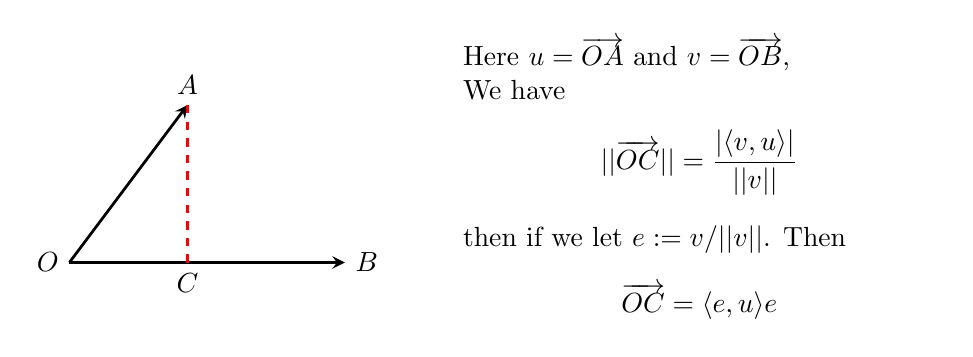
\begin{tikzpicture}[>=stealth,line width=1pt]
        %矩形四个顶点坐标点
        \coordinate [label=left:{$O$}] (O) at (0,0);
        \coordinate [label=above:{$A$}] (A) at (1.5,2);
        \coordinate [label=right:{$B$}] (B) at (3.5,0);
        \coordinate [label=below:{$C$}] (C) at (1.5,0);
        %画箭头:
        \draw[->] (0,0) --+(1.5,2) ;
        \draw[->] (0,0) --+(3.5,0) ;
        \draw[red,dashed] (1.5,2)--(1.5,0) ; 
        \node [below=1cm, align=flush left,text width=6cm] at (8,4)
        {
            Here $u = \overrightarrow{OA}$ and $v = \overrightarrow{OB}$, \\
            We have 
            \[||\overrightarrow{OC}|| = \frac{|\<v,u\>|}{||v||}\]
            then if we let $e:=v/||v||$. Then
            \[\overrightarrow{OC} = \<e,u\>e\]
            
        };
    \end{tikzpicture} 
    So we consider the length of $\overrightarrow{AC}$
    \[
        \begin{aligned}
            ||\overrightarrow{AC}||^{2} &= ||u-\<e,u\>e^{2} = \<u-\<e,u\>e,u-\<e,u\>e\>\\
                                        &= ||u||^{2}-|\<e,u\>|^{2}
        \end{aligned}
    \]
    Since the square is non-negative,
    \[|\<u,v\>|^{2} = ||v||^{2}\cdot |\<u,e\>|^{2} \leq ||u||^{2} \cdot ||v||^{2}.\]
    \end{block}
\end{frame}
\begin{frame}{The Induced Norm}
    \begin{block}{1.3.7. Corollary.}
        The induced norm is actually a norm, i.e., it satisfies 
        \begin{enumerate}[(i)]
            \item $||v|| \geq 0$,$||v|| = 0 \Leftrightarrow v = 0,$
            \item $||\lambda v|| = |\lambda|\cdot||v||,$
            \item $||u+v|| \leq ||u||+||v||$
        \end{enumerate}
        for all $u,v \in V$ and $\lambda \in \F$.
    \end{block}
    \begin{block}{Proof.}
        We only need to check the third property.
        \[
            \begin{aligned}
                ||u+v||^{2} &= ||u||^{2}+||v||^{2}+\<u,v\>+\<v,u\>\\
                &= ||u||^{2}+||v||^{2}+2Re\<u,v\>\\
                &\leq ||u||^{2}+||v||^{2}+2\<u,v\>\\
                &\leq ||u||^{2}+||v||^{2}+2||u||||v||\\
                &= (||u||+||v||)^{2}.
            \end{aligned}
        \]
    \end{block}
\end{frame}
\begin{frame}{Orthogonality}
    \begin{block}{1.3.11. Definition.}
        Let $(V,\<\cdot,\cdot\>)$ be an inner product vector space.
        \begin{enumerate}[(i)]
            \item Two spaces $u,v \in V$ are called \highlightg{orthogonal} or \highlightg{perpendicular} if $<u,v> = 0$
            \item We called
            \[M^{\bot}:=\left\{v\in V:\forall_{m \in M}\<m,v\> = 0\right\}\]
            the \highlightg{orthogonal complement} of a set $M \subset V$.
        \end{enumerate}
        For short, we sometimes write $v \bot M$ instead of $v \in M^{\bot}$ or $v \bot M$ for all $m \in M$.
    \end{block}
    \begin{block}{1.3.12. Lemma.} The orthogonal complement $M^{\bot}$ is a subspace of $V$.
    \end{block}
    \begin{block}{Proof.}
        This result follows the linearity of inner product in definition.
    \end{block}
\end{frame}
\begin{frame}{Orthogonality}
    \begin{block}{Pythagoras's Theorem.}
        Let $(V,\<\cdot,\cdot\>)$ be an inner product space and $M$ some subset of $V$. Let $z = x + y$, where $x \in M$ and $y \in M^{\bot}$. Then
        \[||z||^{2} = ||x||^{2}+||y||^{2}\].
    \end{block}
    \begin{block}{Parallelogram Rule}
        Let $V$ be a real or complex vector space. Then every norm on $V$, if it is induced by some inner product, then it satisfies 
        \[||x+y||^{2}+||x-y||^{2} = 2(||x||^{2}+||y||^{2})\]
        for all $x,y \in V$.
    \end{block}
\end{frame}
\begin{frame}{Orthogonality}
    \begin{block}{Exercise}
        Suppose that $V_{1},...,V_{m}$ are inner product spaces. Show that the equation
        \[\<(u_{1},...,u_{m}),(v_{1},...,v_{m})\> = \<u_{1},v_{1}\>+\cdots+\<u_{m},v_{m}\>\]
        defined an inner product on $V_{1} \times \cdots \times V_{m}$.\\
        Note that for $V_{1},...,V_{m}$, they may have different definition of inner product.
    \end{block}
\end{frame}
\begin{frame}{Orthonorlma Systems}
    \begin{block}{1.3.14. Definition.}
        Let $(V,\<\cdot,\cdot\>)$ be an inner product space. A tuple of vectors $(v_{1},...,v_{r}) \subset V$ is called a \highlightg{(finite) orthonormal system} if 
        \[
            \<v_{j},v_{k}\> = \delta_{jk} :=
            \left\{
                \begin{aligned}
                    1 &\quad \text{for}\ j = k \\
                    0 &\quad \text{for}\ j \neq k \\
                \end{aligned}
            \right.
            \qquad j,k = 1,...,r,
        \] 
        i.e.,if $||v_{k}|| = 1$ and $v_{j} \bot v_{k}$ for $j \neq k$.
    \end{block}
    \begin{block}{1.3.16. Lemma.}
        Let $(V,\<\cdot,\cdot\>)$ be an inner product space and $\mathcal{F} = (v_{1},...,v_{r}) \subset V$ an orthonormal system. Then the elements of $\mathcal{F}$ are linearly independent.
    \end{block}
    \begin{block}{Proof.}
        We assume that $\sum \lambda_{i}v_{i} = 0$, and take inner product of this equation with $v_{i}$. We have $\lambda_{1} = \cdots = \lambda_{r} = 0$.
    \end{block}
\end{frame}
\begin{frame}{Orthonormal Bases}
    \begin{block}{1.3.17. Definition.}
        Let $(V,\<\cdot,\cdot\>)$ be a finite-dimensional inner product vector space and $\mathcal{B} = (e_{1},...,e_{n})$ a basis of $V$. If $\mathcal{B}$ is also an orthonormal system, we say that $\mathcal{B}$ is an \highlightg{orthonormal basis} (ONB).
    \end{block}
    \begin{block}{1.3.18. Theorem.}
        Let $(V,\<\cdot,\cdot\>)$ be a finite-dimensional inner product vector space and $\mathcal{B} = (e_{1},...,e_{n})$ an orthonormal basis of $V$. Then every $v \in V$ has the basis representation
        \begin{spacing}{0.5}
        \[v = \sum_{j = 1}^{n}\<e_{j},v\>e_{j}.\]
        \end{spacing}
    \end{block}
    \begin{block}{1.3.19. Definition.}
        The numbers $\<e_{j},v\>$ are called \highlightg{Fourier coefficients} of $v$ with respect to the basis $\mathcal{B}$. The vector 
        \begin{spacing}{0.7}
        \[\pi_{e_{i}}v:=\<e_{i},v\>e_{i}\]
        \end{spacing}
        is called the \highlightg{projection of $v$ onto $e_{i}$}.
    \end{block}
\end{frame}
\begin{frame}{Orthonormal Bases}
    \begin{block}{Proof of Theorem 1.3.18.}
        Since $\mathcal{B}$ is a basis, for every $v \in V$ it has basis representation
        \begin{spacing}{0.7}
        \[v = \sum_{j = i}^{n}\lambda_{j}e_{j}.\]
        \end{spacing}
        Then we take inner product of this equation with $e_{k}$
        \begin{spacing}{0.7}
        \[\<e_{k},v\> = \sum_{j = 1}^{n}\lambda_{j}\<e_{k},e_j\> = \lambda_{k},\]
        \end{spacing}
        this gives the coefficients of the basis representation.
    \end{block}
    \begin{block}{1.3.20. Parseval's Theorem}
        Let $(V\<\cdot,\cdot\>)$ be a finite-dimensional inner product vector space and $\mathcal{B} = \{e_{1},...,e_{n}\}$ an orthonormal basis of $V$.\\
        Then 
        \[||v||^{2} = \sum_{i = 1}^{n}|\<v,e_{i}\>|^{2}\]
        for any $v \in V$.
    \end{block}
    \begin{block}{Proof.}
        This theorem follows from the basis representation in Theorem 1.3.18. and generalized Pythagoras's Theorem.
    \end{block}
\end{frame}
\begin{frame}{The Projection Theorem}
    \begin{block}{1.3.21. Projection Theorem.}
        Let $(V,\<\cdot,\cdot\>)$ be a (possibly infinite-dimensional) inner product vector space and $(e_{1},...,e_{r}),r \in \N$, be an orthonormal system in $V$. Denote $U:=\text{span}\{e_{1},...,e_{r}\}$.\\
        Then for every $v \in V$ there exists a unique representation
        \begin{spacing}{0.8}
        \[v = u+w \qquad \text{where }u \in U \text{ and } w \in U^{\bot}\]
        \end{spacing}
        and $u = \sum \limits_{i = 1}^{r}\<e_{i},v\>e_{i},\ w:= v-u.$
    \end{block}
    \begin{block}{1.3.22. Definition.}
        The vector
        \[\pi_{U}v:=\sum_{i = 1}^{r}\<e_{i},v\>e_{i}\]
        is called the 
        \highlightg{orthogonal projection of $v$ onto $U$}. Note that $U$ may consist different orthonormal system, but this expression will give the same $\pi_{U}v$ from the uniqueness of the Projection Theorem.
    \end{block}
\end{frame}
\begin{frame}{The Projection Theorem}
    \begin{block}{Proof of the Projection Theorem.}
        We first show the uniqueness of the decomposition: Assume that $v = u+w = u'+w'$. Then by Pythagoras's theorem,
        \[0 = ||u-u'+w-w'||^{2} = ||u-u'||^{2}+||w-w'||^{2}\]
        so $||u-u'|| = ||w-w'|| = 0$. Thus $u = u'$ and $w = w'$.\\
        Now we need to confirm that $u \in U$ and $w \in U^{\bot}$. It is clear that 
        \[u = \sum_{i = 1}^{r}\<e_{i},v\>e_{i}\]
        lies in $U$. So we need to check that $w \in U^{\bot}$.
    \end{block}
\end{frame}
\begin{frame}{The Projection Theorem}
    \begin{block}{Proof of the Projection Theorem(Continued).}
        For this orthonormal basis $\mathcal{B} = (e_{1},...e_{r})$, we have
        \begin{spacing}{0.8}
        \[
            \begin{aligned}
                \<e_{i},v-u\> &= \<e_{i},v\>-\sum_{j = 1}^{r}\<e_{i},e_{j}\>\<e_{j},v\> \\
                &= \<e_{i},v\>-\sum_{j = 1}^{r}\delta_{ij}\<e_{j},v\> \\
                &= \<e_{i},v\>-\<e_{i},v\>\\
                &= 0
            \end{aligned}
        \]
        \end{spacing}
        so $w = v-u$ is orthogonal to an orthonormal basis in $U$. For an arbitrary $u' \in U$ with basis representation $u' = \sum \lambda'_{i}e_{i}$
        \begin{spacing}{0.8}
        \[\<u',w\> = \sum_{i = 1}^{r}\overline{\lambda'}\<e_{i},w\> = 0.\]
        \end{spacing}
        So $w \in U^{\bot}$.
    \end{block}
\end{frame}
\begin{frame}{Orthogonal Subspaces}
    \begin{block}{1.3.24. Corollary.} 
        Let $(V,\<\cdot,\cdot\>)$ be a (possibly infinite-dimensional) inner product vector space and let $U \subset V$ be a finite-dimensional subspace.\\
        Then 
        \[V = U \oplus U^{\bot}\]
        If $V$ is finite-dimensional, then 
        \[\text{dim}V = \text{dim}U + \text{dim}U^{\bot}.\]
        Projection theorem states that $V$ has unique representation with $u \in U$ and $w \in U^{\bot}$, so from Lemma 1.2.27. they are orthogonal and from Theorem 1.2.28. the values of dimension has this relation.
    \end{block}
    \begin{block}{Comment:}
        Note this definition of orthogonality is different from geometrical definition. Two planes in $\R^{3}$ are not orthogonal.
    \end{block}
\end{frame}
\begin{frame}{Bessel's Inequality}
    \begin{block}{1.3.25. Bessel's Inequality.} Let $()V,\<\cdot,\cdot\>)$ be an (possibly infinite-dimensional) inner product space and $(e_{1},...,e_{n})$ and orthonormal system in $V$. Then, for any $v \in V$ and any $r \leq n$,
        \[\sum_{i = 1}^{r}|\<e_{i},v\>|^{2}\leq ||v||^{2}.\]
    \end{block}
    \begin{block}{Proof.}
        From the Projection Theorem and Pythagoras' Theorem 1.3.13 we have $v-u \bot u$, so $||v-u||^{2}+||u||^{2} = ||v||^{2}$, then
        \[0 \leq ||v-u||^{2} = ||v||^{2}-||u||^{2} = ||v||^{2}-\sum_{i = 1}^{r}|\<e_{i},v\>|^{2}.\]
    \end{block}
\end{frame}
\begin{frame}{Best Approxiamtion}
    Using finite number of bases, we cannot express an arbitrary $v \in V$, however, it is possible for us to find the expression that minimizes $||v-u||^{2}$ with $u \in U$, here $u$ has basis representation
    \[
        \begin{aligned}
            ||v-\sum_{i = 1}^{r}\lambda_{i}e_{i}||^{2}&=||v||^{2}+\sum_{i = 1}^{r}|\lambda_{i}|^{2}-\sum_{i = 1}^{r}\lambda_{i}\<v,e_{i}\>-\sum_{i = 1}^{r}\overline{\lambda_{i}}\<e_{i},v\> \\
            &=||v||^{2}+\sum_{i = 1}^{r}(\<e_{i},v\>-\lambda_{i})\overline{(\<e_{i},v\>-\lambda_{i})}-\sum_{i = 1}^{r}|\<e_{i},v\>|^{2}\\
            &=||v||^{2}-\sum_{i = 1}^{r}|\<e_{i},v\>|^{2} +\sum_{i = 1}^{r}|\<e_{i},v\>-\lambda_{i}|^{2}
        \end{aligned}
    \]
    Note the first two terms are constant, and the last term will be 0 if $\lambda_{i} = \<e_{i},v\>,$ i.e., the coefficients are just Fourier coefficients.\\
    If we extend the number of bases from $r$ to $r'$, then 
    \[||v-\sum_{i = 1}^{r'}\<e_{i},v\>e_{i}||\leq||v-\sum_{i = 1}^{r}\<e_{i},v\>e_{i}||\qquad \text{for any } r' \geq r,\]
    the approximation will be better.
\end{frame}
\begin{frame}{Gram-Schmidt Orthonormalization}
    Let $(V,\<\cdot,\cdot\>)$ be an inner product vector space and $(v_{1},...,v_{n})$ is a system of vectors in $V$.\\
    \begin{block}{Motivation:}
        Given a vector $v$, what is the best approximation using this system? Or, what is the best approximate vector in $\text{span}\{v_{1},...,v_{n}\}$?
    \end{block}
    \begin{block}{Solution:}
        An orthonormal system in $\text{span}\{v_{1},...,v_{n}\}$ will give the result by inner product. But an orthonormal system will be arbitrary, what is the most convenient one we can find?
    \end{block}

\end{frame}
\begin{frame}{Gram-Schmidt Orthonormalization}
    We start from $\mathcal{B} = \{v_{1}\}$, and add another normalized vector that is orthogonal to the span of existing basis.
    \begin{enumerate}[(i)]
        \item Normalize $v_{1}$ 
        \[ w_{1} = \frac{v_{1}}{||v_{1}||}, \quad\mathcal{B} = \{w_{1}\}\]
        \item Add the orthogonal part of $v_{2}$ to this system,
        \[v_{2}' = v_{2}-\<w_{1},v_{2}\>w_{1} \in \text{span}\{v_{1}\}^{\bot}\]
        \begin{spacing}{0.02}
        Normalize $v_{2}'$ 
        \[w_{2} = \frac{v_{2}'}{||v_{2}'||},\quad \mathcal{B} = \{w_{1},w_{2}\}\]
        \end{spacing}
        $\vdots$
        \item Add the orthogonal part of $v_{n}$ to this system
        \begin{spacing}{0.3}
        \[v_{n}' = v_{n}-\sum_{i = 1}^{n-1}\<w_{i},v_{n}\>w_{i} \in \text{span}\{w_{1},...,w_{n-1}\}^{\bot}\]
        \end{spacing}
        \vspace{0.5em}
        Normalize $v_{n}'$ 
        \begin{spacing}{0.05}
        \[ w_{n} = \frac{v_{n}'}{||v_{n}'||}, \quad \mathcal{B} = \{w_{1},...,w_{n}\}\]
        \end{spacing}
        \end{enumerate}
\end{frame}
\subsection{Linear Maps}
\begin{frame}{Linear Maps on Vector Spaces}
    \begin{block}{1.4.1. Definition.}
        Let $(U,\oplus,\odot)$ and $(V,\boxplus,\boxdot)$ be vector spaces that are either both real or both complex. Then a map $L:U \rightarrow V$ is said to be \highlightg{linear} if it is both \highlightg{homogeneous} and \highlightg{additive}, i.e.,
        \[L(\lambda \odot u ) = \lambda \boxdot L(u) \quad \text{and} \quad L(u \oplus v) = L(u)\boxplus L(v)\]
        for all $u,v \in U$ and $\lambda \in \F$. The set of all linear maps $L:U \rightarrow V$ is denoted by $\mathcal{L}(U,V)$.
    \end{block}
    \begin{block}{1.4.2. Remark.}
        \begin{enumerate}[(i)]
        \item Note that 
        \[L(0 \oplus 0) = L(0) \boxplus L(0) = L(0)\]
        so $L(0) = 0$. Then we will use same symbol $0$ for the zero in $U$ or in $V$.
        \item The identity map $\text{id}: V \rightarrow V$, $\text{id}(v) = v$, is linear.
        \end{enumerate}
    \end{block}
\end{frame}
\begin{frame}{Linear Maps are Structure-Preserving}
    A linear map
    \[L:U \rightarrow V\]
    between vector spaces $(U,\oplus,\odot)$ and $(V,\boxplus,\boxdot)$ is a \highlightg{structure-preserving map}.\\
    Note that the composition of linear maps will still be linear, i.e., if $L_{1} \in \mathcal{L}(U,V)$ and $L_{2} \in \mathcal{L}(V,W)$, then $L_{1} \circ L_{2} \in \mathcal{L}(U,W)$.\\
    We assume that $L$ is bijective such that $L^{-1}$ exists. Then for a linear map $\sigma:V \rightarrow V$, we can define $\pi:U \rightarrow U,$
    \[\pi = L^{-1} \circ \sigma \circ L\]
    since $L$ and $\sigma$ are linear, the new function $\pi$ is also a linear map.
    \begin{center}
    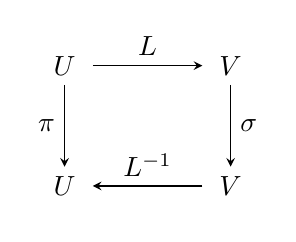
\begin{tikzpicture}
        \matrix (m) [ampersand replacement =\&, matrix of math nodes,row sep=3em,column sep=4em,minimum width=2em]
        {
           U \& V \\
           U \& V \\};
        \path[-stealth]
          (m-1-1) edge node [left] {$\pi$} (m-2-1)
                  edge node [above] {$L$} (m-1-2)
          (m-1-2) edge node [right] {$\sigma$} (m-2-2)
          (m-2-2) edge node [above] {$L^{-1}$} (m-2-1);
    \end{tikzpicture}
    \end{center}
\end{frame}
\begin{frame}{Comments on Structure-Preserving}
    \begin{block}{Other thoughts....}
        Here you see a formula that will appear frequently in your further study:
        \begin{shrinkeq}{-0.3em}
        \[z = L^{-1} \circ x \circ L\]
        \end{shrinkeq}
        One interpretation is:\\
        \textit{The operation on one space is done by another operation on another space.}\\
        A similar formula has appeared before, recall that the projection of vector $v$ on a normal vector $e$ is 
        \begin{shrinkeq}{-0.5em}
        \[\pi_{e} = \<e,v\>e\]
        \end{shrinkeq}
        You will further understand that a vector is a linear map $e:\F \rightarrow \F^{n}$, and the inner product $\<e,\cdot\>$ is the adjoint.\\
        If $\text{span}\{v\} \neq \text{span}\{e\}$, and a function $f:\text{span}\{v\} \rightarrow \text{span}\{e\}$ is linear, such that 
        \begin{shrinkeq}{-0.3em}
        \[f(\lambda v) = \lambda f(v)\]
        \end{shrinkeq}
        then $f$ will be a multiple of $\pi_{e}$.
    \end{block}
\end{frame}
\begin{frame}{Homomorphisms and Finite-Dimensional Spaces}
    \begin{block}{1.4.4. Theorem.}
        Let $U,V$ be real or complex spaces. If $(b_{1},...,b_{n})$ is a basis in $U$, then for every $(v_{1},...,v_{n}) \in V^{n}$, there exists a unique linear map $L:U \rightarrow V$ such that $Lb_{k} = v_{k}$, $k = 1,...,n$.\\
        Note that we assume $\text{dim}U = n$ but $V$ can be infinite-dimensional.
    \end{block}
    \begin{block}{Proof.}
        \structb{(Uniqueness)} Assume another linear map $M \in \mathcal{L}(U,V)$ with $Mb_{k} = v_{k}$.\\
        For any $u \in U$, $u = \sum \lambda_{k}b_{k}$,
        \[
            \begin{aligned}
                Lu &= L(\sum \lambda_{k}b_{k}) = \sum \lambda_{k}L(b_{k}) \\
                &= \sum \lambda_{k} v_{k} = \sum \lambda_{k} M(b_{k}) = M(\sum \lambda_{k} v_{k}) = Mu.
            \end{aligned}
        \]
        so $Lu = Mu$ for any $u \in U$, we then have $L = M$.
    \end{block}
\end{frame}
\begin{frame}{Homomorphisms and Finite-Dimensional Spaces}
    \begin{block}{Proof(Continued).}
        \structb{(Existence)} We define the linear map for $u \in U$, $u = \sum \lambda_{k}b_{k}$,
        \[Lu:=\sum \lambda_{k}v_{k}\]
        We need to check this is a linear map. If $u,u' \in U$ are $u = \sum \lambda_{k}b_{k}$ and $u' = \sum \lambda_{k}b_{k}$, we have
        \[L(u+u') = \sum (\lambda_{k}+\lambda_{k}')v_{k} = \sum \lambda_{k}v_{k}+ \sum \lambda_{k}'v_{k} = Lu+Lu'\]
        Let $\mu \in \F$,
        \[L(\mu u) = L(\sum \mu \lambda_{k}v_{k}) = \sum \mu \lambda_{k}v_{k} = \mu \sum \lambda_{k}v_{k} = \mu L(u)\]
        so this is a linear map.
    \end{block}
\end{frame}
\begin{frame}{Coordinate Map and Dual Space}
    \begin{block}{}
        \structb{1.4.6. Examples.} Let $V$ a real or complex vector space, and $(b_{1},...,b_{n})$ be a basis of $V$ if it is finite-dimensinonal.
        \begin{enumerate}[(i)]
            \item If $\text{dim}V = n$, the \highlightg{corrdinate map}
            \begin{spacing}{0.6}
            \[
                \varphi:V \rightarrow \F^{n}, \qquad v = \sum \lambda_{k}b_{k} \mapsto 
                \begin{pmatrix}
                    \lambda_{1}\\
                    \vdots\\
                    \lambda_{n}\\
                \end{pmatrix}
            \]
            \end{spacing}
            is linear (and bijective).
            \item Then $\mathcal{L}(V,\F)$ is known as the \highlightg{dual space} of $V$ and denoted by $V^{*}$. \\
            If $\text{dim}V = n$, then we can find a basis of the dual space $V^{*}$,
            \begin{spacing}{0.8}
            \[
                b_{k}^{*}:V \rightarrow \F,
                \qquad
                b_{k}^{*}(b_{j}) = \delta_{jk}.
            \]
            \end{spacing}
            Note that if $V^{*}$ is an inner product space, then 
            \begin{spacing}{0.7}
            \[b_{k}^{*} = \<b_{k},\cdot\>\]
            \end{spacing}
            can express the basis in $V^{*}$. 
        \end{enumerate}
    \end{block}
\end{frame}
\begin{frame}{Range and Kernel}
    \begin{block}{1.4.8. Definition.}
        Let $U,V$ be real or complex vector spaces and $L \in \mathcal{L}(U,V)$. Then we define the \highlightg{range} of $L$ by
        \begin{spacing}{0.8} 
        \[\text{ran}L:=\left\{v \in V:\exists_{u \in U}v = Lu\}\right.\]
        \end{spacing}
        and the \highlightg{kernel} of $L$ by
        \begin{spacing}{0.8}
        \[\text{ker}L:=\left\{u \in U:Lu = 0\}\right. \]
        \end{spacing}
        We can notice that $\text{ran}L \subset V$ and $\text{ker}L \subset U$ are subspaces.
    \end{block}
    \begin{block}{1.4.9. Remark.}
        For $L \in \mathcal{L}(U,V)$, it is injective if and only if $\text{ker}L = \{0\}.$\\
    \structb{Proof.}
    \begin{spacing}{0.4}
        \[
            \begin{aligned}
                L\text{ is injective }  
                & \Leftrightarrow 
                Lx = Ly \ \Rightarrow\ x = y, \text{ for any }x,y \in V \\
                & \Leftrightarrow
                L(x-y) = 0 \ \Rightarrow\ x-y = 0, \text{ for any }x,y \in V\\
                & \Leftrightarrow
                Lu = 0 \ \Rightarrow\ u = 0, \text{ for any }u \in V\\
                & \Leftrightarrow
                \text{ker}L = \{0\}.
            \end{aligned}
        \]
    \end{spacing}
    \end{block}
\end{frame}
\begin{frame}{Range and Kernel}
    \begin{block}{Digression.}
        Let $U,V$ be vector spaces with $\text{dim}U = n$. For a basis $(b_1,...,b_{n}) \in U$, and we define $L$ by a $n$-tuple $(Lb_{1},...,Lb_{n}) \in V$, then what are $\text{ran}L$ and $\text{ker}L$?
    \end{block}
    \begin{block}{Solution.}
        We apply Gram-Schmidt to $(Lb_{1},...,Lb_{n})$ and apply the same linear combinations on $(b_{1},...,b_{n})$.\\
        Then
        \[
            \begin{aligned}
                (Lb_{1},...,Lb_{n}) \xrightarrow{Gram-Schmidt} (c_{1},...,c_{r},0,...,0)\\
                (b_{1},...,b_{n}) \xrightarrow{\text{Same Linear Combinations}} (b_{1}',...,b_{n}')\\
            \end{aligned}
        \]
        here $(c_{1},...,c_{r})$ is an orthonormal basis.
        Then we get 
        \[
            \begin{aligned}
                \text{ran}L = \text{span}\{c_{1},...,c_{r}\}\\
                \text{ker}L = \text{span}\{b_{r+1}',...,b_{n}'\}.\\
            \end{aligned}
        \]
    \end{block}
\end{frame} 
\begin{frame}{Nomenclature}
    Fancy names for linear maps. A homomorphism $L \in \mathcal{L}(U,V)$ is 
    \begin{itemize}
        \item an \highlightg{isomorphism} if $L$ is bijective (isos means "equal");
        \item an \highlightg{endomorphism} if $U = V$;
        \item an \highlightg{automorphism} if $U = V$ and $L$ is bijective;
        \item \highlightg{epimorph} if $L$ is surjective;
        \item \highlightg{monomorph} if $L$ is injective;
    \end{itemize}
    \begin{block}{Comments:}
        Possibly only two terms will occur again...\\
        \structb{Isomorphism} $L$ "relabels" elements from $U$ to $V$, such that they have the same structure.\\
        \structb{Homomorphism} $L$ partly preserves the structure from $U$ to $V$.\\
        Prof. Zach McKenzie likes these two terms very much, you will see them frequently in Discrete Math (if you are ECE major), such as group homomorphism, lattice homomorphism, and graph isomorphism...
    \end{block}
\end{frame}
\begin{frame}{Isomorphisms}
    \begin{block}{1.4.11. Theorem.}
        Let $U,V$ be finite-dimensional vector spaces and $L \in \mathcal{L}(U,V)$. Then $L$ is an isomorphism if and only if every basis $(b_{1},...,b_{n})$ of $U$, the tuple $(Lb_{1},...,Lb_{n})$ is a basis of $V$.
    \end{block}
    \begin{block}{Proof.}
        \structb{$(\Rightarrow)$} Assume that $L$ is bijective. For $y \in V$, there will be unique $x = L^{-1}y \in U$ because $L$ is bijective. And $x = \sum \lambda_{k}b_{k}$ is the unique basis representation in $U$. Now
        \[y = L(\sum \lambda_{k}b_{k}) = \sum \lambda_{k} \cdot Lb_{k}\]
        so $y$ has unique representation using $(Lb_{1},...,Lb_{n})$. Then $(Lb_{1},...,Lb_{n})$ is a basis in $V$, from the \highlightr{original definition}.\\
    \end{block}
\end{frame}
\begin{frame}{Isomorphisms}
    \begin{block}{Proof(Continued).}
        \structb{$(\Leftarrow)$} Note the the coordinate map will be a bijection, so 
        $\varphi:U \rightarrow \F^{n}$ with basis $(b_{1},...,b_{n})$ and $\phi:V \rightarrow \F^{n}$ with basis $(Lb_{1},...,Lb_{n})$ are bijections. Then from Theorem 1.4.4. $L = \phi^{-1} \circ \varphi$ are the same map, then $L$ is a bijection from $U$ to $V$ since the composition of bijections will still be a bijection.
    \end{block}
    \begin{block}{1.4.12. Definition.} Two vector spaces $U$ and $V$ are called \highlightg{isomorphic}, written $U \cong V$, if there exists an isomorphism $\varphi:U \rightarrow V$.
    \end{block}
    \begin{block}{1.4.13. Lemma.} Two finite-dimensional vector spaces $U$ and $V$ are isomorphic if and only if they have the same dimension:
    \begin{spacing}{0.5}
        \[U \cong V \qquad \Leftrightarrow \qquad \text{dim}U = \text{dim}V\]
    \end{spacing}
    \end{block}
    \begin{block}{Proof.}
        $L$ is isomorphism
        $\Leftrightarrow$ $(b_{1},...,b_{n})$ and $(Lb_{1},...,Lb_{n})$ are basis.
    \end{block}
\end{frame}
\begin{frame}{The Dimension Formula}
    \begin{block}{1.4.14. Dimension Formula.}
        Let $U,V$ be real or complex vector spaces, $\text{dim}U < \infty$. Let $L \in \mathcal{L}(U,V)$. Then 
        \[\text{dim}\ \text{ran}L+\text{dim}\ \text{ker}L = \text{dim}U.\]
    \structb{Proof.}\\
        Let $\text{dim}U = n$, and $\text{dim}\ \text{ker}L = r$, $(a_{1},...,a_{r})$ is a basis of $\text{ker}L$.\\
        By Basis Extension Theorem, we can find $(a_{1},...,a_{r},a_{r+1},...,a_{n})$ is a basis in $U$.\\
        We want to show that $L$ is a bijection from $\text{span}\{a_{r+1},...,a_{n}\}$ to $\text{ran}L$. \highlightr{(We change the domain of this function)}\\
        \structb{(1)Surjection.} For $y \in \text{ran}L$, there exists $x \in U$, with $x = \sum \lambda_{k}a_{k}$, $Lx = y$. Because 
        \begin{spacing}{0.7} 
        \[
            y = Lx = L(\lambda_{1}a_{1}+\cdots+\lambda_{n}a_{n}) = \lambda_{r+1}La_{r+1}+ \cdots +\lambda_{n}La_{n},
        \]
        \end{spacing}
        we have $z = \lambda_{r+1}a_{r+1}+\cdots+\lambda_{n}a_{n} \in \text{span}\{a_{r+1},...,a_{n}\}$, with $Lz = y$. 
    \end{block}
\end{frame}
\begin{frame}{The Dimension Formula}
    \begin{block}{Proof(Continued).}
        \structb{(2)Injection.} If for $y \in \text{ran}L$, there are $Lx = Lx' = y$ with $x = \sum_{k = r+1}^{n} \lambda_{k}a_{k}$ and $x = \sum_{k = r+1}^{n} \lambda_{k}'a_{k}$, then $L(x-x') = 0$ means $x-x' \in \text{ker}L$, so we have
        \[(\lambda_{r+1}-\lambda_{r+1}')a_{r+1}+\cdots+(\lambda_{n}-\lambda_{n}')a_{n} = \eta_{1}a_{1}+\cdots+\eta_{r}a_{r}.\]
        We have $(a_{1},...,a_{n})$ is a basis, so $\lambda_{k} = \lambda_{k}'$ for $k = r+1,...,n$.
    \end{block}
    \begin{block}{1.4.15. Corollary.}
        Let $U,V$ be real or complex finite-dimensional vector spaces with $\text{dim}U = \text{dim}V$. Then a linear map $L \in \mathcal{L}(U,V)$ is injective if and only if it is surjective.\\
    \structb{Proof.}\\
       We notice that $\text{ker}L = \{0\}$ are $\text{ran}L = V$ are equivalent.
    \end{block}
\end{frame}
\begin{frame}{Normed Vector Spaces and Bounded Linear Maps}
    \begin{block}{1.4.16. Definition.}
        Let $(U,||\cdot||_{U})$ and $(V,||\cdot||_{V})$ be normed vector spaces. Then a linear map $L:U \rightarrow V$ is said to be \highlightg{bounded} if there exists some constant $c > 0$ (called a \highlightg{bound} for $L$) such that
        \begin{spacing}{0.7} 
        \[||Lu||_{V} \leq c \cdot ||u||_{U}\qquad \text{for all }u \in U.\]
        \end{spacing}
    \end{block}
    \begin{block}{1.4.18. Examples.}
        The map $\int:C([a,b])\rightarrow \R$ definite integral is a bounded map.
        \[\int_{a}^{b}f \leq |b-a| \cdot \sup_{x \in [a,b]}|f(x)|\]
        Note that continuous function is bounded on $[a,b]$, so $\sup_{x \in [a,b]}$ exists. Here the norm of $C((a,b))$ is $\sup_{x \in [a,b]}|\cdot|$.\\
        \structb{Question:}
        Will it still be bounded with a different norm?
    \end{block}
\end{frame}
\begin{frame}{Bounded Linear Maps}
    \begin{block}{1.4.17. Remark.}
        If $U$ is finite-dimensional vector space, then any linear map is bounded.
    \end{block}
    \begin{block}{Proof.}
        Consider $(b_{1},...,b_{n})$ is a basis in $U$, then for $u \in U$, with $u = \sum \lambda_{k}b_{k}$,
        \[
            \begin{aligned}
                \|Lu\|_{V} &\leq |\lambda_{1}|\|Lb_{1}\|_{V}+\cdots+|\lambda_{n}|\|Lb_{n}\|_{V}\\
                &\leq n \cdot \max_{k = 1,...,n}|\lambda_{k}\||Lb_{k}\|_{V}\\
                &\leq n \cdot \|u\|_{U}.
            \end{aligned}
        \]
        So every liner map is bounded.
    \end{block}       
\end{frame}
\begin{frame}{The Operator Norm}
    \begin{block}{1.4.19. Definition and Theorem.}
        Let $U,V$ be normed vector spaces. Then the set of bounded linear maps $\mathcal{L}(U,V)$ is also a vector space and 
        \[\|L\|:=\sup_{u \in U,\,u \neq 0}\frac{\|Lu\|_{V}}{\|u\|_{U}} = 
        \sup_{u \in U,\,\|u\|_{U} = 1}\|Lu\|_{V}.\]
        defines a norm, the so-called \highlightg{operator norm} or \highlightg{induced norm} on $\mathcal{L}(U,V)$.
    \end{block}
    \begin{block}{Proof.}
        This is a norm since $\|\cdot\|_{V}$ is a norm, for each $\|u\|_{V} = 1$,
        \begin{spacing}{0.7}
        \[\|Lu\| \geq 0, \text{ and }\|Lu\| = 0 \Rightarrow Lu = 0\]
        \end{spacing}
        so $\sup\|Lu\|_{V} \geq 0$ and $\sup\|Lu\|_{V} = 0$ iff $Lu = 0$ for any $u \in U$.\\
        We also have
        \begin{shrinkeq}{-2ex}
        \[
            \sup\|\lambda Lu\|_{V} = |\lambda| \cdot \sup\|Lu\|_{V},\ 
            \sup\|Lu+L'u\| \leq \sup\|Lu\|+\sup\|L'u\|
        \]
        \end{shrinkeq}
    \end{block}
\end{frame}
\begin{frame}{The Operator Norm}
    \begin{block}{Theorem.}
        The operator norm has the additional property that
        \[\|L_{2}L_{1}\| \leq \|L_{2}\| \cdot \|L_{1}\|, \qquad L_{1} \in \mathcal{L}(U,V), \qquad L_{2}\in \mathcal{L}(V,W).\]
    \end{block}
    \begin{block}{Proof.}
        From definition
        \[
            \begin{aligned}
                \|L_{2}L_{1}\| 
                &= \sup_{u \in U,\ \|u\|_{U} = 1}\|L_{2}L_{1}u\|\\
                &\leq \sup_{u \in U,\ \|u\|_{U} = 1}\left(\sup_{v \in V,\ \|v\|_{V} = 1}\|L_{2}v\| \cdot \|L_{1}u\|\right)\\
                &= \sup_{v \in V,\ \|v\|_{V} = 1}\|L_{2}v\| \cdot \sup_{u \in U,\ \|u\|_{U} = 1} \|L_{1}u\|\\
                &= \|L_{2}\|\cdot\|L_{1}\|.
            \end{aligned}
        \]
    \end{block}
\end{frame}
\subsection{Matrices}
\begin{frame}{A Calculus of Linear Maps}
    The word \highlightg{calculus} means a "scheme of calculating".\\
    \begin{block}{Motivation}
        Recall Theorem 1.4.4., a linear map from $U$ to $V$ can be determined by a basis $(b_{1},...,b_{n})$ in $U$ and $(Lb_{1},...,Lb_{n})$ in $V$.\\
         We want to find a good notation to "store" these information.
    \end{block}
    \begin{block}{Solution}
        For finite-dimensional case, we notice that if $\text{dim}U = n$ and $\text{dim}V = m$, we can find isomorphism $\varphi_{1}:U \rightarrow \R^{n}$ and $\varphi_{2}:V \rightarrow \R^{m}$. For linear maps from $\R^{n}$ to $\R^{m}$, we can write them down using \highlightg{matrices}.
    \end{block}
    \begin{block}{Comment:}
            We are supposed to replace $\R$ by $\F$ here since $U$ and $V$ may be complex.
    \end{block}
\end{frame} 
\begin{frame}{Matrices}
    \begin{block}{1.5.1. Definition.}
        An matrix is a map
        \[a:\{1,...,m\}\times\{1,...,n\} \rightarrow \F,\qquad (i,j) \mapsto a_{ij}.\]
        And it can be represented by a graph
        \[A:=
        \begin{pmatrix}
            a_{11} & \cdots & a_{1n}\\
            \vdots & \ddots & \vdots \\
            a_{m1} & \cdots & a_{mn}\\
        \end{pmatrix}
        \]
        We denote all $m \times n$ matrix over $\F$ by $\text{Mat}(m \times n;\F)$. We often write $\C$ or $\R$ instead of $\F$. 
    \end{block}
\end{frame}
\begin{frame}{Matrices as Linear Maps}
    \begin{block}{1.5.3. Theorem.}
        For $A \in \text{Mat}(m \times n;\F)$ and $(e_{1},...,e_{n})$ is the standard basis in $\F^{n}$, then we define $j:\Mat(m \times n;\F) \rightarrow \L(\F^{n},\F^{m})$ by 
        \begin{spacing}{0.7}
        \[
            (e_{1},...,e_{n}) \rightarrow (Le_{1},...,Le_{n}) = (a_{\cdot 1},...,a_{\cdot n})\]
        \end{spacing}
        finding $L$ that satisfies this condition. Then $j(A) = L$ is an isomorphism, and $\Mat(m \times n;\F) \cong \L(\F^{n},\F^{m})$.  
    \end{block}
    \begin{block}{Proof.}
        From Theorem 1.4.4., $L$ is unique and $j$ is a function.\\
        \structb{(1)Injection.} If $j(A) = j(A')$, then each column are the same, so $A = A'$.\\
        \structb{(2)Surjection.} For each $L \in \L(\F^{m},\F^{n})$, there exists $(Le_{1},...,Le_{n})$, so $j$ is a surjection.\\
    \end{block}
    \begin{block}{Comment:}
        Be very careful that a matrix is defined on \highlightg{standard basis}.\\
        We will replace $L$ by $A$ since $j$ is a bijection.
    \end{block}
\end{frame}
\begin{frame}{Matrices as Linear Maps}
    \begin{block}{Calculation Method.}
    For $x \in \F^{n}$,
    \begin{spacing}{0.5}
    \[x = 
    \begin{pmatrix}
        x_{1}\\
        \vdots\\
        x_{n}\\
    \end{pmatrix}
    = 
    x_{1}
    \begin{pmatrix}
        1\\
        0\\
        \vdots\\
        0
    \end{pmatrix}
    +\cdots+
    x_{n}
    \begin{pmatrix}
        0\\
        \vdots\\
        0\\
        1\\
    \end{pmatrix}
    = \sum_{k = 1}^{n}x_{k}e_{k}.
    \]
    \end{spacing}
    then $Ax$ is 
    \begin{spacing}{0.5}
    \[
        \begin{aligned}
            Ax &= A\sum_{k = 1}^{n}x_{k}e_{k}
     = \sum_{k = 1}^{n}x_{k}Ae_{k}
     = \sum_{k = 1}^{n}x_{k}a_{\cdot k}\\
     &=
     x_{1}
     \begin{pmatrix}
        a_{11}\\
        \vdots\\
        a_{m1}\\
     \end{pmatrix}
     +\cdots+
     x_{n}
     \begin{pmatrix}
        a_{1n}\\
        \vdots\\
        a_{mn}\\
     \end{pmatrix}
     =
     \begin{pmatrix}
        x_{1}a_{11}+\cdots+x_{n}a_{1n}\\
        \cdots\\
        x_{1}a_{m1}+\cdots+x_{m}a_{mn}\\
     \end{pmatrix}
    \end{aligned}
    \]
    \end{spacing}
    \end{block}
    \begin{block}{Comment:}
        The last expression looks like inner product on $\F^{n}$ and rows of $A$ are involved.
    \end{block}
\end{frame}
\begin{frame}{Composition and Matrix Product}
    \begin{block}{1.5.4. Definition and Theorem.}
    If $A \in \Mat(l \times m;\F)$ and $B \in \Mat(m \times n;\F)$, then we define the composition of $A$ and $B$ as the \highlightg{product of A and B} by
    \begin{shrinkeq}{-0.7em} 
    \[AB \in \Mat(l \times n;\F), \qquad AB:=\left(\sum_{k = 1}^{m}a_{ik}b_{kj}\right)_{\substack{i = 1,...,l\\j = 1,...,n}}\]
    \end{shrinkeq}
    \end{block}
    \begin{block}{Proof.}
        We need to check that $AB$ is the composition of $A$ and $B$.\\
        The composition of $A$ and $B$ is supposed to have $n$ columns, and $ABe_{j}$ is the $j$th column,
        \begin{shrinkeq}{-0.7em}
        \[ABe_{j} = Ab_{j} = \sum_{k = 1}^{m}a_{\cdot k}b_{kj}\]
        \end{shrinkeq}
        so the entry on $i$th row and $j$th column is 
        \begin{shrinkeq}{-0.7em}
        \[(AB)_{i,j} = \sum_{k = 1}^{m}a_{ik}b_{kj}.\]
        \end{shrinkeq}
    \end{block}
\end{frame}
\begin{frame}{Matrix Product}
    \begin{block}{Comment on matrix product:}
        From composition of linear maps, the product is associative but not commutative.\\
    \end{block}
    \begin{block}{Example.}
        Calculate the matrix product,
        \begin{spacing}{0.7}
        \[
            \begin{pmatrix}
                1 & 0 & 0 & 0 \\
                -1 & 1 & 0 & 0 \\
                0 & -1 & 1 & 0 \\
                0 & 0 & -1 & 1 \\
            \end{pmatrix}
            \begin{pmatrix}
                0 & 0 & 0 & 1 \\
                0 & 0 & 1 & 1 \\
                0 & 1 & 1 & 1 \\
                1 & 1 & 1 & 1 \\
            \end{pmatrix}
        \]
        \end{spacing}
    \end{block}
    \begin{block}{Question:}
        What is the result for general case?
    \end{block}
\end{frame}
\begin{frame}{Vectors are Matrices}
    \begin{block}{Motivation.}
        Note that vectors in $\F^{n}$ is written as a map $u:\{1\} \times \{1,...,n\} \rightarrow \F$, which is exactly a $n \times 1$ matrix. So what is the linear map it represents?
    \end{block}
    \begin{block}{Solution.}
        From the definition of matrices, we know that $u \in \L(\F,\F^{n})$. So it maps $1$ to $u$.
    \end{block}
    \begin{block}{Comment:}
        So there are three interpretation of a vector in $\F^{n}$, a vector, a matrix and a linear map. We have three vector spaces are isomorphic,
        \[\F^{n} \cong \Mat(n \times 1,\F) \cong \L(\F,\F^{n}).\]
        For finite-dimensional vector space with $\text{dim}V = n$, we can replace $\F^{n}$ by $V$.
    \end{block}
\end{frame}
\begin{frame}{Matrices of Inner Product}
    \begin{block}{Motivation.}
        We have shown that for $v \in V$, $\<v,\cdot\>$ is a linear map in $\L(V,\F)$, so what is the matrix of this linear map?
    \end{block}
    \begin{block}{Solution.}
        Assume that $\text{dim}V = n$ and $(e_{1},...,e_{n})$ is a standard basis in $V$. If $v^{*}$ is the matrix of $\<v,\cdot\>$, then 
        \[v^{*} = (\<v,e_{1}\>,...,\<v,e_{n}\>) = (\overline{\<e_{1},v\>},...,\overline{\<e_{n},v\>}) = (\overline{v_{1}},...,\overline{v_{n}}).\]
        Note that we transfer a linear map $v \in \L(\F,V)$ to a linear map $v^{*} \in \L(V,\F)$. 
    \end{block}
    \begin{block}{Comment:}
        This result shows that 
        \[V^{*} = \L(V,\F) \cong \Mat(1 \times n;\F).\]
    \end{block}
\end{frame}
\begin{frame}{The Matrix of the Adjoint of a Linear Map}
    \begin{block}{Motivation.}
    Recall that 'dual' is means a map that reverses the domain and the codomain, so what is $T^{*}$ that corresponds to $T \in \L(U,V)$? 
    \begin{center}
    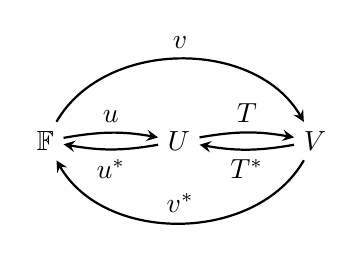
\begin{tikzpicture}[node distance = 1.2cm]
        \node (F) {$\F$};
        \node (U) [right = of F] {$U$};
        \node (V) [right = of U] {$V$};
        \draw [->,thick] (F) to [in = 170, out=10]node[pos=.5,above] {$u$} (U) ;
        \draw [->,thick] (U) to [in = 170, out=10]node[pos=.5,above] {$T$} (V) ;
        \draw [->,thick] (F) to [in=120,out=60] node[pos=.5,above] {$v$} (V) ;
        
        \draw [->,thick] (U) to [in = -10,out = -170]node[pos=.5,below] {$u^{*}$} (F) ;
        \draw [->,thick] (V) to [in = -10,out = -170]node[pos=.5,below] {$T^{*}$} (U) ;
        \draw [->,thick] (V) to [in=-60,out=-120] node[pos=.5,above] {$v^{*}$} (F) ;
    \end{tikzpicture}
    \end{center}
    We can determine $T^{*}$ from this diagram, if $A$ is the matrix of $T$, 
        \begin{center}
            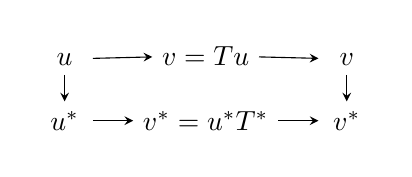
\begin{tikzpicture}
                \matrix (m) [ampersand replacement = \&, matrix of math nodes,row sep=1em,column sep=1.5em, minimum width = 2em]
                {
                    u \& v = Tu \& v \\
                    u^{*} \& v^{*} = u^{*}T^{*} \&v^{*}\\ 
                };
                \path[-stealth]
                (m-1-1) edge (m-1-2)
                (m-1-2) edge (m-1-3)
                (m-1-1) edge (m-2-1)
                (m-1-3) edge (m-2-3)
                (m-2-1) edge (m-2-2)
                (m-2-2) edge (m-2-3);
            \end{tikzpicture}
        \end{center}
        we want to find the matrix of $T^{*}$ denoted $A^{*}$.
        \end{block}
\end{frame}
\begin{frame}{The Matrix of the Adjoint of a Linear Map}
    \begin{block}{Solution.}
        The relation between $T$ and $T^{*}$ is
        \begin{shrinkeq}{-0.3em} 
        \[(Tu)^{*} = u^{*}T^{*},\]
        \end{shrinkeq}
        we transfer $T$ to $A$, $u \in U$ to $x \in \F^{n}$ with $x = \sum x_{i}e_{i}$.\\
        \structb{(1)Left} From the additivity of dual,  
        \[(Ax)^{*} = \sum_{i =1}^{n}(x_{i}a_{\cdot i})^{*} = \sum_{i = 1}^{n}\overline{x_{i}}a_{\cdot i}^{*},\]
        here $a_{\cdot i}^{*}$ is the dual of $a_{\cdot i}$ in $\L(\F^{n},\F)$.\\ 
        \structb{(2)Right}
        Assume that the matrix of $T^{*}$ is $A' \in \Mat(n \times m;\F)$, when we take $e_{j} \in \F^{m}$,(Sorry using $A^{*}$ directly may be misleading...)
        \[x^{*}A'e_{j} = x^{*}a'_{\cdot j} = \<x,a'_{\cdot j}\>,\]
    \end{block}
\end{frame}
\begin{frame}{The Matrix of the Adjoint of a Linear Map}
    \begin{block}{Solution(Continued).}
        so
        \begin{spacing}{0.5}
        \begin{shrinkeq}{-0.5em}
        \[
            \begin{aligned}
                x^{*}A' &= (\<x,a'_{\cdot 1}\>,...,\<x,a'_{\cdot m}\>) 
                &= 
        \left(
            \begin{array}{c}
                \overline{x_{1}}a'_{11}\\
                +\\
                \vdots\\
                +\\
                \overline{x_{n}}a'_{n1}\\
            \end{array},...,
            \begin{array}{c}
                \overline{x_{1}}a'_{1m}\\
                +\\
                \vdots\\
                +\\
                \overline{x_{n}}a'_{nm}\\
            \end{array}
        \right)
        &=\sum_{i = 1}^{n}\overline{x_{i}}a'_{i \cdot}
        \end{aligned}
        \]
        \end{shrinkeq}
        \end{spacing}
        \structb{(3)Left equals right,}
        \begin{shrinkeq}{-0.3em}
        \[(Ax)^{*} = \sum_{i = 1}^{n}\overline{x_{i}}a_{\cdot i}^{*} = x^{*}A' = \sum_{i = 1}^{n} \overline{x_{i}}a'_{i \cdot}\]
        \end{shrinkeq}
        so we have 
        \begin{shrinkeq}{-0.5em}
        \[a_{\cdot i}^{*} = a'_{i \cdot}\]
        \end{shrinkeq}
        we will replace $A'$ by $A^{*}$ afterwards. This means that \\
        \begin{center}
        \textit{The rows of $A^{*}$ are the dual of columns of $A$.}
        \end{center}
    \end{block}
\end{frame}
\begin{frame}{Adjoint of a Linear Map}
    \begin{block}{Definition.}
        Let $U,V$ be vector spaces and $T \in \L(U,V)$, then the adjoint of $T$ denoted $T^{*} \in \L(V,U)$ is the unique linear map that satisfies,
        \[\<Tu,v\> = \<u,T^{*}v\>\]
        for any $u \in U$, $v \in V$.
    \end{block}
    \begin{block}{Comment:}
        Note that this definition is the same as the previous result,
        \[\<Tu,v\> = (Tu)^{*}v = u^{*}T^{*}v = \<u,T^{*}v\>.\]
    \end{block}
\end{frame}
\begin{frame}{Matrix Transpose}
    \begin{block}{Definition.}
        For $A = (a_{ij}) \in \Mat(m \times n;\F)$ we define the \highlightg{transpose} of $A$ by 
        \[A^{T} \in \Mat(n \times m;\F),\ A^{T} = (a_{ji}).\]
    \end{block}
    \begin{block}{Theorem.}
        The \highlightg{adjoint} of a matrix is 
        \[A^{*} \in \Mat(n \times m;\F),\ A^{*} = \overline{A}^{T} = (\overline{a_{ji}}).\]
    \end{block}
\end{frame}
\begin{frame}{Matrix Transpose}
    We stated that adjoint is the "dual" of a linear map. However, the dual map is defined as follows.
    \begin{block}{Definition and Theorem.}
        If $T \in \L(U,V)$, then the \highlightg{dual map} of $T$ is the linear map $T' \in \L(V^{*},U^{*})$ defined by $T'(v^{*}) = v^{*} \circ T$ for $v^{*} \in V$.\\
        If $(b_{1},...,b_{n})$ is a basis of $U$ and $(c_{1},...,c_{m})$ is a basis of $V$, with 
        \[
            \begin{aligned}
                \varphi_{A1}(b_{1},...,b_{n}) = \varphi_{A2}(b_{1}^{*},...,b_{n}^{*}) = (e_{1},...,e_{n})\\
                \varphi_{B1}(c_{1},...,c_{m}) = \varphi_{B2}(c_{1}^{*},...,c_{m}^{*}) = (e_{1},...,e_{m}),\\
            \end{aligned}
        \]
        we have the matrix of $T$ is $A$ and the matrix of $T'$ is $A'$, then
        \[A' = A^{T}.\]
    \end{block}
\end{frame}
\begin{frame}{Matrix Transpose}
    \begin{center}
        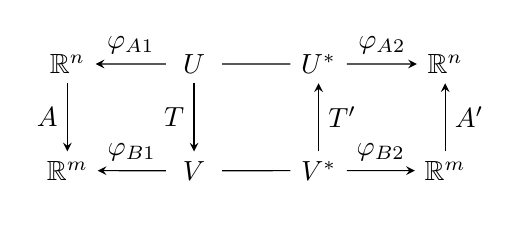
\begin{tikzpicture}
            \matrix (m) [ampersand replacement =\&, matrix of math nodes,row sep=2.5em,column sep=2.5em,minimum width=2em]
            {
               \R^{n} \& U \& U^{*} \& \R^{n} \\
               \R^{m} \& V \& V^{*} \& \R^{m} \\};
            \path[-stealth]
              (m-1-1) edge node [left] {$A$} (m-2-1)
              (m-1-2) edge node [above] {$\varphi_{A1}$} (m-1-1)
              (m-2-2) edge node [above] {$\varphi_{B1}$} (m-2-1)
              (m-1-2) edge node [left] {$T$} (m-2-2)
              (m-2-3) edge node [right] {$T'$}
              (m-1-3)
              (m-1-3) edge node [above] {$\varphi_{A2}$} (m-1-4)
              (m-2-4) edge node [right] {$A'$} (m-1-4)
              (m-2-3) edge node [above] {$\varphi_{B2}$} (m-2-4);
            \path (m-1-2) edge (m-1-3)
            (m-2-2) edge (m-2-3);
        \end{tikzpicture}
    \end{center}
    \begin{block}{Proof.}
        Each column of $A'$ is 
        \[
            \begin{aligned}
                A'e_{j} &= \varphi_{A2} \circ T' \circ \varphi_{B2}^{-1}e_{j}\\
                &= \varphi_{A2} \circ T' (c_{j}^{*})\\
                &= \varphi_{A2} \circ (c_{j}^{*} \circ T),\\
            \end{aligned}
        \]
        we use $T'(v^{*}) = v^{*} \circ T$ here.
    \end{block}
\end{frame}
\begin{frame}{Matrix Transpose}
    \begin{block}{Proof(Continued).}
        To calculate $c_{j}^{*} \circ T$, we notice that 
        \[c_{j}^{*} \circ T = c_{j}^{*} \circ \varphi_{B1}^{-1} \circ A \circ \varphi_{A1}.\]
        From the left, $c_{j}^{*} \circ \varphi_{B1}^{-1} = e_{j}^{*}$ since its product with basis are the same. From previous result we know that, 
        \[e_{j}^{*}A = a_{j\cdot}.\]
        Then we have 
        \[A'e_{j} = \varphi_{A2} \circ a_{j\cdot} \circ \varphi_{A1}.\]
    \end{block}
\end{frame}
\begin{frame}{Matrix Transpose}
    \begin{block}{Proof(Continued).}
        We consider that 
        \[
            \begin{aligned}
                a_{j \cdot} \circ \varphi_{A1} &= \sum_{i = 1}^{n}a_{ji}e_{i}^{*}\varphi_{A1} \\
                &= \sum_{i = 1}^{n}a_{ji}b_{i}^{*}.\\
            \end{aligned} 
        \]
        In the last step we used $e_{i}^{*}\varphi_{A1} = b_{i}^{*}$ similar to $c_{j}^{*}\circ\varphi_{B1}^{-1} = e_{j}^{*}$. Finally we have
        \[
            \begin{aligned}
                A'e_{j} &= \varphi_{A2}\sum_{i = 1}^{n}a_{ji}b_{i}^{*}\\
                &= \sum_{i = 1}^{n}a_{ji}e_{i}.
            \end{aligned}
        \]
        We have $A' = (a_{ji}) = A^{T}$ as the result.
        \end{block}
    \end{frame}
\begin{frame}{Properties of Adjoint}
    \begin{block}{Theorem.}
        Let $U,V$ be vector spaces. If $T \in \L(U,V)$ and $T^{*} \in \L(V,U)$, then
        \[
            \begin{aligned}
                (\text{ran}T)^{\bot} = \text{ker} T^{*} \\
                (\text{ran}T^{*})^{\bot} = \text{ker} T.
            \end{aligned}
        \]
        \end{block}
        \begin{block}{Proof.}
            Note that $v \in (\text{ran}T)^{\bot}$ is 
            \[(\forall u \in U)\<Tu,v\> = 0 \quad \Leftrightarrow \quad (\forall u \in U)\<u,T^{*}v\> = 0,\]
            the second statement is only possible for $T^{*}v = 0$, then $v \in \text{ker}T^{*}.$
        \end{block}
        \end{frame}
        \begin{frame}{Properties of Adjoint}
            \begin{block}{Comment:}
                Note that this theorem can be expressed as,
            \[
                \begin{aligned}
                    \text{ran}T\oplus\text{ker}T^{*} = V,\\
                    \text{ran}T^{*}\oplus\text{ker}T = U.\\
                \end{aligned}
            \]
                If $U,V$ are finite-dimensional,
            \[
            \begin{aligned}
                \text{dim } \text{ran}T+\text{dim } \text{ker}T^{*} = \text{dim}V\\
                \text{dim } \text{ran}T^{*}+\text{dim } \text{ker}T = \text{dim}U.\\
            \end{aligned}
            \]
        \end{block}
        \end{frame}
        \begin{frame}{Properties of Adjoint}
            \begin{block}{Motivation.}
                For vector spaces $U,V$, we have $T \in \L(U,V)$. Then we can find $\text{ran}T$ and $\text{ker}T$, so we can determine $\text{ran}T^{*} = (\text{ker}T)^{\bot}$ and $\text{ker}T^{*} = (\text{ran}T)^{\bot}$. Can we express $T^{*}$ using basis of these subspaces?
            \begin{center}
                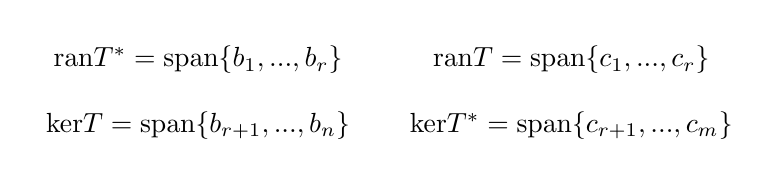
\begin{tikzpicture}
                    \matrix (m) [ampersand replacement = \&, matrix of math nodes,row sep=0.7em,column sep=1.5em, minimum width = 2em]
                    {
                        \text{ran}T^{*} = \text{span}\{b_{1},...,b_{r}\} \& \text{ran}T = \text{span}\{c_{1},...,c_{r}\} \\
                        \text{ker}T = \text{span}\{b_{r+1},...,b_{n}\} \& \text{ker}T^{*} = \text{span}\{c_{r+1},...,c_{m}\}\\ 
                    };
                \end{tikzpicture}
            \end{center}
            If $T(b_{i}) = c_{i}$ for $i = 1,...,r$, then is $T^{*}(c_{i}) = b_{i}$ the adjoint of $T$?
        \end{block}
    \end{frame}
    \begin{frame}{Properties of Adjoint}
        \begin{block}{Solution.}
            We only have this result for suitable basis. If $u = \sum_{i = 1}^{n}\lambda_{i}b_{i}$ and $v = \sum_{j = 1}^{m}\mu_{j}c_{j}$, then 
            \[
                \begin{aligned}
                    \<Tu,v\> &= \<T\sum_{i = 1}^{n}\lambda_{i}b_{i},\sum_{j = 1}^{m}\mu_{j}c_{j}\> = \<\sum_{i = 1}^{r}\lambda_{i}c_{i},\sum_{j = 1}^{m}\mu_{j}c_{j}\> \\
                \end{aligned}
            \]
            since we have $\text{span}\{c_{1},...,c_{r}\} \bot \text{span}\{c_{r+1},...,c_{n}\}$. 
            \[
                \begin{aligned}
                    \<Tu,v\> &= \<\sum_{i = 1}^{r}\lambda_{i}c_{i},\sum_{j = 1}^{r}\mu_{j}c_{j}\>+\<\sum_{i = 1}^{r}\lambda_{i}c_{i},\sum_{j = r+1}^{m}\mu_{j}c_{j}\>\\
                    &=\<\sum_{i = 1}^{r}\lambda_{i}c_{i},\sum_{j = 1}^{r}\mu_{j}c_{j}\>.
                \end{aligned}
            \]
            \end{block}
        \end{frame}
        \begin{frame}{Properties of Adjoint}
            \begin{block}{Solution(Continued).}
            The same result for adjoint
            \[\<u,T^{*}v\> = \<\sum_{i = 1}^{r}\lambda_{i}b_{i},\sum_{j = 1}^{r}\mu_{j}b_{j}\>,\]
            so we have 
            \[\<\sum_{i = 1}^{r}\lambda_{i}c_{i},\sum_{j = 1}^{r}\mu_{j}c_{j}\> = \<\sum_{i = 1}^{r}\lambda_{i}b_{i},\sum_{j = 1}^{r}\mu_{j}b_{j}\>.\]
            Because $\lambda_{i}$ and $\mu_{j}$ are arbitrary, we have 
            \[\<b_{i},b_{j}\> = \<c_{i},c_{j}\> \qquad i,j = 1,...,r.\]
            With basis that satisfies this equation, we can have for $T(b_{i}) = c_{i}$ the adjoint is $T^{*}(c_{i}) = b_{i}.$
        \end{block}
    \end{frame}
    \begin{frame}{Second Way to Understand Matrix times Vector}
        Recall that a matrix times a vector has results look like inner product, and we explain this using adjoint. For $A \in \Mat(m \times n;\F)$, $x \in \F^{n}$,
        \[
            Ax = (x^{*}A^{*})^{*} = (\<x,a_{\cdot 1}^{*}\>,...,\<x,a_{\cdot m}^{*}\>)^{*},
        \]
        here $a_{\cdot i}^{*}$ is the $i$th column of $A^{*}$.\\
        \begin{spacing}{0.7}
        \[Ax = 
        \begin{pmatrix}
            \overline{\<x,a_{\cdot 1}^{*}\>}\\
            \vdots\\
            \overline{\<x,a_{\cdot m}^{*}\>}\\
        \end{pmatrix} = 
        \begin{pmatrix}
            \<a_{\cdot 1}^{*},x\>\\
            \vdots\\
            \<a_{\cdot m}^{*},x\>\\
        \end{pmatrix} =
        \begin{pmatrix}
            a_{1 \cdot}x\\
            \vdots\\
            a_{m \cdot}x\\
        \end{pmatrix}
        \]
    \end{spacing}
        We have proved that the rows of $A^{*}$ are the dual of columns of $A$, then the rows of $A$ are the dual of the columns of $A^{*}$.\\
        In the last step, we use
        \begin{shrinkeq}{-0.3em}
        \[a_{i \cdot} = \<a_{\cdot i}^{*}, \cdot\>,\]
        \end{shrinkeq}
        the final result is matrix product between $a_{i \cdot}$ and $x$.
\end{frame}
\begin{frame}{Dimension of $U \times V$ and $\L(U,V)$}
    \begin{block}{Theorem.}
        Let $U,V$ be real or complex finite-dimensional vector spaces. For $\text{dim}U = n$ and $\text{dim}V = m$,
        \begin{shrinkeq}{-0.5em}
        \[
            \begin{aligned}
                \text{dim}(U \times V) = n+m \\
            \end{aligned}
        \]
        \end{shrinkeq}
        Note that $\L(U,V) = n \times m$ since matrix has $n \times m$ independent entries.
    \end{block}
    \begin{block}{Proof.}
        For a basis $(b_{1},...,b_{n})$ in $U$ and a basis $(c_{1},...,c_{m})$ in $V$, we find a basis in $U \times V$ by 
        \[((b_{1},0),...,(b_{n},0),(0,c_{1}),...,(0,c_{m}))\]
        Note that for $u \in U$, $u = \sum \lambda_{k}b_{k}$ and for $v \in V$, $v = \sum \mu_{j}c_{j}$, so 
        \[(u,v) = \sum \lambda_{k}(b_{k},0)+ \sum \mu_{j}(0,c_{j})\]
        is the unique representation, $\dim(U \times V) = n+m$.
    \end{block}
\end{frame}
\begin{frame}{Block Matrix}
    \begin{block}{Motivation.}
        If we have two linear maps $L_{1} \in \L(U,W)$ and $L_{2} \in \L(V,W)$, can we define $L \in \L(U \times V,W)$? \\
        In other way, if we have $L_{1} \in \L(U,V)$ and $L_{2} \in \L(U,W)$, can we define $L \in \L(U,V \times W)$?
    \end{block}
    \begin{block}{Solution.}
        If we have the matrix of $L_{1},L_{2}$ are $A,B$, and the matrix of $L$ is $C$. Then in the first situation,
        \begin{spacing}{0.7}
        \[C = 
        \begin{pmatrix}
            A & B\\
        \end{pmatrix}.
        \]
        \end{spacing}
        In the second situation,
        \begin{spacing}{0.7}
        \[C = 
        \begin{pmatrix}
            A\\
            B\\
        \end{pmatrix}.
        \]
    \end{spacing}
        This method gives rise to block matrix.
    \end{block}
\end{frame}
\begin{frame}{Block Matrix}
    \begin{block}{Properties.}
        From definition, we can simplify the result when matrices times from left,
        \begin{spacing}{0.7}
        \[T
        \begin{pmatrix}
           A & B\\
        \end{pmatrix} = 
        \begin{pmatrix}
            TA & TB\\
        \end{pmatrix}.
        \]
    \end{spacing}
        Then from right,
        \begin{spacing}{0.7}
        \[
            \begin{pmatrix}
                A\\
                B\\
            \end{pmatrix}
            T = 
            \begin{pmatrix}
                AT\\
                BT\\
            \end{pmatrix}.
        \]
        \end{spacing}
    \end{block}
\end{frame}

\begin{frame}{Elementary Matrix Manipulations}
    When we apply Gauss-Jordan Algorithm to solve a linear system, we use three types of linear maps in matrix form.
    \begin{block}{Definition.}
        For a linear system $Ax = b$ with $b \in \F^{m}$ and $A \in \Mat(m \times n;\F)$, we have three types of elementary matrices:
        \begin{enumerate}
            \item Row switching. 
            \begin{shrinkeq}{-0.3em}
            \[a_{i \cdot} \leftrightarrow a_{j \cdot},\]
            \end{shrinkeq}
            \item Row multiplications.
            \begin{shrinkeq}{-0.3em}
            \[ka_{i \cdot} \rightarrow a_{i\cdot}, \ \text{where}k \neq 0,\]
            \end{shrinkeq}
            \item Row addition.
            \begin{shrinkeq}{-0.3em}
            \[a_{i\cdot}+ka_{j\cdot} \rightarrow a_{i\cdot}.\] 
            \end{shrinkeq}
        \end{enumerate}
    \end{block}
    \begin{block}{Comment:}
        Note that $\text{ran}A^{*}$ does not change, then $\text{ker}A$ which is $(\text{ran}A^{*})^{\bot}$ does not change.
    \end{block}
\end{frame} 
\begin{frame}{Inverse of a Matrix}
    If $A \in \Mat(n \times n;\F)$, we find the inverse map of $A$ by solving linear system $Ax = b$.
    \begin{block}{1.5.9. Definition.}
        A matrix $A \in \Mat(n \times n;\F)$ is called \highlightg{invertible} if there exists some $B \in \Mat(n \times )$ such that 
        \begin{spacing}{0.5}
        \[AB = BA = \text{id} = 
        \begin{pmatrix}
            1 & & 0\\
              & \ddots & \\
              0 & & 1
        \end{pmatrix}.\]
        \end{spacing}
        We then write $B = A^{-1}$ and say that $A^{-1}$ is the \highlightg{inverse} of $A$.
    \end{block}
    \begin{block}{Comment:}
        If $BA = \text{id}$, then
        \begin{shrinkeq}{-0.3em} 
        \[AB = A \cdot\text{id} \cdot B = A(BA)B =(AB)(AB),\]
        \end{shrinkeq}
        so $AB = \text{id}$.
    \end{block}
\end{frame}
\begin{frame}{Find the Inverse}
    \begin{block}{Gauss-Jordan Algorithm}
        For $A \in \Mat(m \times n;\F)$, we write it in juxtaposition with the identity matrix and apply the Gauss-Jordan Algorithm to them at the same time, then 
        \begin{spacing}{0.7}
        \[B
        \begin{pmatrix}
            A & \text{id} 
        \end{pmatrix}
        = 
        \begin{pmatrix}
           \text{id} & \text{B} 
        \end{pmatrix}.
        \]
    \end{spacing}
        So we get $B$ is $A^{-1}$.
        Here $B$ is the multiplication of all elementary matrices.
    \end{block}
\end{frame}
\begin{frame}{Inverse Maps}
    Recall that to express a linear map $L \in \L(U,V)$ with $\dim U = n,\dim V = m$, we need two bijections $\varphi_{A} \in \L(U,\F^{n})$ and $\varphi_{B} \in \L(V,\F^{m})$. Then we can determine the matrix $A \in \Mat(m \times n;\F)$ such that 
    \[L = \varphi_{B} \circ A \circ \varphi_{A}.\]
    \begin{block}{Solution.}
        To express the inverse of isomorphism $L \in \L(U,V)$ with $\dim U = \dim V = n$, we have 
        \[L^{-1} = \varphi_{A}^{-1} \circ A^{-1} \circ \varphi_{B}^{-1},\]
        where $A^{-1}$ is the inverse of $A$.
    \end{block}
\end{frame}
\begin{frame}{Inverse Maps}
    \begin{block}{Examples.}
        For $L:\mathcal{P}_{2} \mapsto \mathcal{P}_{2}$, such that 
        \[ax^{2}+bx+c \mapsto \frac{a+b+c}{3}x^{2}+\frac{a+b}{2}x+\frac{a-c}{2}.\]
        with
        \[
            \begin{aligned}
                \varphi_{A}:\mathcal{P}_{2} \mapsto \F^{3}, \qquad \varphi_{A}(1,x,x^{2}) = (e_{1},e_{2},e_{3})\\
                \varphi_{B}:\mathcal{P}_{2} \mapsto \F^{3}, \qquad \varphi_{B}(1,x,x^{2}) = (e_{1},e_{2},e_{3})
            \end{aligned} 
        \]
        find $L^{-1}$ with $\varphi_{A}^{-1},\varphi_{B}^{-1}$.
    \end{block}
    \begin{block}{Comment:}
        Different $\varphi_{A},\varphi_{B}$ will not change the expression of $L^{-1}$.
    \end{block}
\end{frame} 
\begin{frame}{Linear Maps - Active and Passive Points of View}
    We only consider $2D$ case as in class, take $T(e_{1},e_{2}) = (b_{1},b_{2})$.
    \begin{block}{Active.}
        When we apply $T$ to $x \in \R^{2}$, we find 
        \[Tx = T(x_{1}e_{1}+x_{2}e_{2}) = x_{1}b_{1}+x_{2}b_{2}.\]
    \end{block}
    \begin{block}{Passive.}
        For $x \in \R^{2}$, 
        \[x = T^{-1}Tx = T^{-1}(x_{1}b_{1}+x_{2}b_{2}),\]
        so $T^{-1}$ acts on it without changing it.
    \end{block}
\end{frame}
\begin{frame}{Change of Basis}
    We need to express $x$ using basis $(e_{1}',...,e_{n}')$ if we have known the standard representation.
    \begin{block}{Active.}
        We write down the matrix of $T$ such that $T(e_{1},...,e_{n}) = (e_{1}',...,e_{n}')$.
        We have two representations of $x$,
        \begin{shrinkeq}{-0.3em}
        \[x = \sum_{i = 1}^{n}x_{i}e_{i} = \sum_{i = 1}^{n}x_{i}'e_{i}',\]
        \end{shrinkeq}
        then apply $T^{-1}$ on both sides,
        \begin{shrinkeq}{-0.3em}
        \[T^{-1}\sum_{i = 1}^{n}x_{i}e_{i} = \sum_{i = 1}^{n}x_{i}'T^{-1}e_{i}' = \sum_{i = 1}^{n}x_{i}'e_{i},\]
        \end{shrinkeq}
        so $T^{-1}x$ has coordinate coefficients equal to $x_{i}'$.
    \end{block}
    \begin{block}{Comment:}
        We solve a linear system here, we denote $x' = \sum_{i = 1}^{n}x_{i}'e_{i}'$, then $x = Tx'$, so $x' = T^{-1}x$.
    \end{block}
\end{frame}
\begin{frame}{Change of Basis}
    We applied linear map and found another vector, but we can find the matrix of basis change directly as well.
    \begin{block}{Passive.}
        We consider $\text{id}:\R^{2} \rightarrow \R^{2}$, take 
        \begin{shrinkeq}{-0.3em}
        \[
            \begin{aligned}
                \varphi_{A}(e_{1},e_{2}) = (e_{1},e_{2})\\
                \varphi_{B}(e_{1}',e_{2}') = (e_{1},e_{2})\\
            \end{aligned}
        \]
        \end{shrinkeq}
        Then $x' = Ax$ where $x' = x_{1}'e_{1}+x_{2}'e_{2}$ and $x = x_{1}e_{1}+x_{2}e_{2}$.
        \begin{center}
            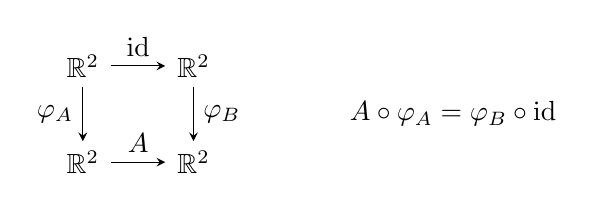
\begin{tikzpicture}
                \matrix (m) [ampersand replacement =\&, matrix of math nodes,row sep=2em,column sep=2em,minimum width=2em]
                {
                   \R^{2} \& \R^{2} \\
                   \R^{2} \& \R^{2} \\};
                \path[-stealth]
                  (m-1-1) edge node [left] {$\varphi_{A}$} (m-2-1)
                          edge node [above] {id} (m-1-2)
                  (m-1-2) edge node [right] {$\varphi_{B}$} (m-2-2)
                  (m-2-1) edge node [above] {$A$} (m-2-2); 
                  \node (T) at (4,0) {$A \circ \varphi_{A} = \varphi_{B} \circ \text{id}$};
            \end{tikzpicture}
        \end{center}
            Note that $\varphi_{A} = \text{id},\varphi_{B} = T^{-1}$, then $A = T^{-1}$.
        \end{block}
    \end{frame}
    \begin{frame}{Reflection in $\R^{2}$}
        The reflection matrix with respect to x-axis is 
        \begin{spacing}{0.5}
        \[A = 
        \begin{pmatrix}
            1 & 0\\
            0 & -1\\
        \end{pmatrix}
            \]
    \end{spacing}
        \begin{block}{Example.}
            Find the matrix of the linear map $L:\R^{2} \rightarrow \R^{2}$ such that it takes reflection of a vector with respect to the line through
            \begin{spacing}{0.5}
            \[y = 
            \begin{pmatrix}
                1 \\
                2 \\
            \end{pmatrix}.\]
        \end{spacing}
    \end{block}
\end{frame}
\begin{frame}{Reflection in $\R^{2}$}
    \begin{block}{Solution.}
        We consider the basis 
        \begin{spacing}{0.5}
        \[b_{1} = \begin{pmatrix}
            1\\
            2\\
        \end{pmatrix},b_{2} = \begin{pmatrix}
            2\\
            -1\\
        \end{pmatrix}.\]
    \end{spacing}
    If $x = \lambda_{1}b_{1}+\lambda_{2}b_{2}$, then 
    \[Lx = \lambda_{1}b_{1}-\lambda_{2}b_{2},\]
    so we define $T(e_{1},e_{2}) = (b_{1},b_{2})$, then 
    \[L = TAT^{-1},\]
    we use basis change in previous slide.
\end{block}
\end{frame}

\begin{frame}{Structure of Solution Sets}
    \begin{block}{Motivation.}
        For linear system $Ax = b$, the solution set $S$ is not a subspace, so how to express $S$?
    \end{block}
    \begin{block}{Sloution.}
        Note that if $x_{1},x_{2} \in S$, then $A(x_{2}-x_{1}) = 0$, and $x_{2}-x_{1} \in \text{ker}A$. If $Ax_{p} = b$, then 
        \[x_{p}+\text{ker}A:=\{x \in \text{ker}A:x_{p}+x\}\]
        is the solution set $S$. We have to find two things to solve this system, a particular solution $x_{p}$, a basis of $\text{ker}A$.
    \end{block}
\end{frame}
\subsection{Theory of Systems of Linear Equations}
\begin{frame}{Solution Sets}
    \begin{block}{Defitions.}
        \structb{Solution Set} For a linear systems of equations $Ax = b$, the \highlightg{solution set} is 
        \[\text{Sol(A,b)} = \{x \in \R^{n}:Ax = b\}.\]
        \structb{Particular Solution} If $x_{0} \in \R^{n}$ satisfies
        \[Ax_{0} = b ,\]
        then we say that $x_{0}$ is a \highlightg{particular solution} of $Ax = b$.\\
        \structb{Associated homogeneous solution set} 
        \[\text{Sol}(A,0) = \{x \in \R^{n}:Ax = 0\} = \text{ker}A.\]
    \end{block}
\end{frame}
\begin{frame}{Structure of Solution Set}
    A very important, fundamental result states:\\
    \textit{The solution set of $Ax = b$ is the sum of the homogeneous solution set and a particular solution.}
    \begin{block}{1.6.1. Lemma.}
        Let $x_{0} \in \R^{n}$ be a particular solution of $Ax = b$. Then
        \begin{shrinkeq}{-0.3em}
        \[\text{Sol}(A,b) = \{x_{0}\}+\text{ker}A = \left\{y \in \R^{n}:y = x_{0}+x,x \in \text{ker}A \right\}.\]
        \end{shrinkeq}
    \end{block}
    \begin{block}{Proof.}
        Note that for $x \in \R^{n}$, we have 
        \[x \in \text{Sol}(A,b) \Leftrightarrow x-x_{0} \in \text{ker}A.\]
    \end{block}
\end{frame}
\begin{frame}{Solvability of Systems of Equations}
    \begin{block}{1.6.2. Corollary}
        If $x_{0}$ is a particular solution of $Ax = b$ and $\{v_{1},...,v_{r}\}$ is a basis of $\text{ker}A$, then
        \[\text{Sol}(A,b) = \left\{x \in \R^{n}:x = x_{0}+\lambda_{1}v_{1}+\cdots+\lambda_{r}v_{r}:\lambda_{1},...,\lambda_{r} \in \R\right\}.\]
        Here $r = \text{dim ker} A$.
    \end{block}
    \begin{block}{1.6.3. Corollary.} 
        If we have a solution to the linear system of equations $Ax = b$, this solution is unique if and only if $\text{ker}A = \{0\}.$\\
        \structb{Proof.} We have
        \[\text{Sol}(A,b) = \{x_{0}\} \Leftrightarrow \text{ker}A = \{0\}.\]
    \end{block}
\end{frame}
\begin{frame}{Solvability of Systems of Equations}
    This gives rise to a further, fundamentally important result:
    \begin{block}{1.6.4. Fredholm Alternative.}
        Let $A \in \Mat(n \times n;\R^{n})$. Then
        \begin{itemize}
            \item either $Ax = b$ has a unique solution for any $b \in \R^{n}$
            \item or $Ax = 0$ has a non-trivial solution.
        \end{itemize}
    \end{block}
    \begin{block}{Proof.}
        If $A$ is bijective, then $x = A^{-1}b$;\\
        If $A$ is not bijective, it is not injective, then $\text{ker}A \neq \{0\}$.
    \end{block}
    \begin{block}{Comment:}
        This result is only for $A \in \Mat(n \times n)$. For $A \in \Mat(n \times m)$, $A$ is injective is equivalent to $A$ is surjective.
    \end{block}
\end{frame}
\begin{frame}{Matrix Rank}
    \begin{block}{1.6.5. Definition.}
        Let $A \in \Mat(m \times n;\F)$ be a matrix columns $a_{\cdot j}$, $1 \leq j \leq n$, and rows $a_{i \cdot} \in \F^{n}$, $1 \leq i \leq m$. Then we define
        \begin{itemize}
            \item the \highlightg{column rank} of $A$ to be 
            \[\text{column rank }A:=\dim \text{span}\{a_{\cdot 1},...,a_{\cdot n}\}\]
            \item and the \highlightg{row rank} of $A$ to be 
            \[\text{row rank }A:=\dim \text{span}\{a_{1 \cdot},...,a_{m \cdot}\}.\]
        \end{itemize}
    \end{block}
    \begin{block}{1.6.6. Remarks.}
        \begin{itemize}
            \item $\text{row rank }A = \text{column rank }A^{T}$
            \item $\text{column rank }A = \dim \text{ran }A$
        \end{itemize}
    \end{block}
\end{frame}
\begin{frame}{Matrix Rank}
    \begin{block}{1.6.7. Definition and Theorem.}
        Let $A \in \Mat(m \times n;\F)$. Then the column rank is equal to the row rank and we define the \highlightg{rank} of $A$ by
        \begin{shrinkeq}{-0.3em} 
        \[\text{rank} A:=\text{column rank}A = \text{row rank}A.\]
        \end{shrinkeq}
    \end{block}
    \begin{block}{Proof.}
        Recall that $\overline{A}^{T} = A^{*}$, we assume that $\dim \text{ran}\overline{A}^{T} = \dim \text{ran}A^{T}$ and $\dim \text{ker}\overline{A}^{T} = \dim \text{ker}A^{T}$ here, then 
        \begin{shrinkeq}{-0.3em}
        \[
            \begin{aligned}
                \dim \text{ran}A+\dim \text{ker}A^{T} = m\\
                \dim \text{ran}A^{T}+\dim \text{ker}A^{T} = m.\\
            \end{aligned}
        \]
        \end{shrinkeq}
        We subtract these two equations and have
        \begin{shrinkeq}{-0.3em} 
        \[\dim \text{ran}A = \dim \text{ran}A^{T},\]
        \end{shrinkeq}
        so $\text{row rank}A = \text{column rank}A$.
        \end{block}
    \end{frame}
    \begin{frame}{Matrix Rank}
        \begin{block}{Questions:}
            Why $\dim \text{ran}A^{T} = \dim \text{ran}\overline{A}^{T}$?
        \end{block}
        \begin{block}{Answer:}
            If we have $(b_{1},...,b_{r})$ is a basis of $\text{ran}A^{T}$, we state that $(\overline{b_{1}},...,\overline{b_{r}})$ is basis of $\text{ran}\overline{A}^{T}$. For $x \in \text{ran}\overline{A}^{T}$,
            \begin{shrinkeq}{-0.3em}
            \[x = \sum_{i = 1}^{m}\lambda_{i}\overline{a_{i\cdot}}^{T},\]
            \end{shrinkeq}
            then $\overline{x} \in \text{ran}A^{T}$ and we have 
            \[\overline{x} = \sum_{i = 1}^{m}\overline{\lambda_{i}}a_{i\cdot}^{T} = \sum_{j = 1}^{r}\mu_{j}b_{j}.\]
        \end{block}
    \end{frame}
    \begin{frame}{Matrix Rank}
        \begin{block}{Answer(Continued).}
            Note that we have $\mu_{j}$ are unique since $b_{j}$ are basis, then 
            \[x = \sum_{j = 1}^{r}\overline{\mu_{j}}\overline{b_{j}}\]
            is the unique expression with $\overline{b_{j}}$, here we use the fact that $\overline{(\cdot)}$ is a bijection from $\C$ to $\C$. This is true for $x \in \text{ran}\overline{A}^{T}$, then $(\overline{b_{1}},...,\overline{b_{r}})$ is a basis.
        \end{block}
        \begin{block}{Comment:}
            Note that $\overline{(\cdot)}$ is not an isomorphism, but $(\overline{b_{1}},...,\overline{b_{r}})$ is still a basis. 
        \end{block}
    \end{frame}
    \begin{frame}{Existence of Solutions}
        \begin{block}{1.6.8. Theorem.}
            There exists a solution for $Ax = b$ if and only if $\text{rank}A = \text{ran}(A|b)$, where
            \begin{spacing}{0.5}
            \[
                (A|b) = 
                \begin{pmatrix}
                    a_{11} & \cdots & a_{1n} & b_{1} \\
                    \vdots & & \vdots & \vdots\\
                    a_{m1} & \cdots & a_{mn} & b_{m}\\
                \end{pmatrix}
                \in \Mat((n+1) \times m).
            \]
            \end{spacing}
            \end{block}
            \begin{block}{Proof.}
                If $Ax = b$ has a solution we have
                \[b \in \text{ran}A \Leftrightarrow \text{ran}A = \{b\}+\text{ran}A.\]
                Note that $\text{rank}A = \dim \text{ran}A$ and $\text{rank}(A|b) = \dim \left(\{b\}+\text{ran}A\right)$ we have
                \[\text{rank}A = \text{rank}(A|b).\]
            \end{block}
        \end{frame}
\subsection{Determines}
\begin{frame}{The Determinant in $\R^{2}$}
    \begin{block}{Motivation.}
        We want to find the area of a parallelogram spanned by $a$ and $b$,
        \[P(a,b) = \left\{x \in \R^{2}:x = \lambda a+\mu b,0 \leq \lambda \leq 1,0 \leq \mu \leq 1\right\}.\]
    \end{block}
    \begin{block}{Solution.}
        This map is a bilinear map,
        \[\text{det}:\R^{2} \times \R^{2} \rightarrow \R\]
        with properties,
        \begin{enumerate}
            \item $\text{det}(e_{1},e_{2}) = 1$,
            \item $\text{det}(\lambda a,b) = \lambda \text{det}(a,b)$, $\text{det}(a+c,b) = \text{det}(a,b)+\text{det}(c,b)$,
            \item $\text{det}(a,a) = 0$.
        \end{enumerate}
    \end{block}
\end{frame}
\begin{frame}{The Determinant in $\R^{2}$}
    \begin{block}{Solution(Continued).}
        The last property is true for vectors in parallel, it can be extended to 
        \[
            \text{det}(a,b) = -\text{det}(b,a)
        \]
        So for $a = a_{1}e_{1}+a_{2}e_{2}$, $b = b_{1}e_{1}+b_{2}e_{2}$,
        \[
            \begin{aligned}
                \text{det}(a,b) = &a_{1}b_{1}\text{det}(e_{1},e_{1})+a_{1}b_{2}\text{det}(e_{1},e_{2})+\\
                &a_{2}b_{1}\text{det}(e_{2},e_{1})+a_{2}b_{2}\text{det}(e_{2},e_{2})\\
                = &a_{1}b_{2}-a_{2}b_{1}.
            \end{aligned}
        \]
        We then find the area of $P(a,b)$ to be,
        \[A(a,b) = |a_{1}b_{2}-a_{2}b_{1}|.\]
        \end{block}
    \end{frame}
    \begin{frame}{Vector Product in $\R^{3}$}
        We then define the vector product in $\R^{3}$ as,
        \begin{enumerate}
            \item Length, $|a \times b| = A(a,b)$.
            \item Direction, $a \times b\  \bot\  \text{span}\{a,b\}.$
            \item Orientation, $(a,b,a \times b)$ should form a "right-hand system".
        \end{enumerate}
        We can define a map $\times:\R^{3} \times \R^{3} \rightarrow \R^{3}$.
        Note that since in $\R^{n}$ for $n > 3$, $\dim (\text{span}\{a,b\})^{\bot} \geq 1$, so we cannot define vector product.
    \end{frame}
    \begin{frame}{The Determinant in $\R^{3}$}
        \begin{block}{Motivation.}
            We want to find the area of a parallel epiped spanned by three vectors $a,b,c \in \R^{3}$.
        \end{block}
        \begin{block}{Solution.}
            We have the determinant in $\R^{3}$ as an \highlightg{oriented volume},
            \[\text{det}:\R^{3}\times\R^{3}\times\R^{3}, \qquad \text{det}(a,b,c) = \<a \times b,c\>.\]
            Note that previous three properties are preserved.
        \end{block}
    \end{frame}
    \begin{frame}{The Determinant in $\R^{n}$}
        \begin{block}{1.7.13. Definition.}
            A function $f:\R^{n}\times \cdots \times \R^{n} \rightarrow \R$ is said to be a \highlightg{p-multilinear map} (or \highlightg{p-multilinear form}) if $f$ is linear in each entry, i.e.,
            \begin{shrinkeq}{-0.3em}
            \[f(\lambda a_{1},a_{2},...,a_{p}) = \lambda f(a_{1},a_{2},...,a_{p})\]
            \end{shrinkeq}
            and
            \begin{shrinkeq}{-0.3em}
            \[f(a_{1}+b,a_{2},...,a_{p}) = f(a_{1},a_{2},...,a_{p})+f(b,a_{2},...,a_{p})\]
            \end{shrinkeq}
            for $b,a_{1},...,a_{p} \in \R^{n}$ and $\lambda \in \R$ and analogously hold for the other entries.
        \end{block}
        \begin{block}{Definition.}
            A $p-multilinear form $ is said to be \highlightg{alternating} if $f(a_{1},...,a_{p}) = 0$ whenever $a_{j} = a_{k}$ for any $j \neq k$.\\
            It is said to be \highlightg{normed} if $f(e_{1},...,e_{n}) = 1$, where $e_{1},...,e_{n}$ are the standard basis vectors in $\R^{n}$.
        \end{block}
    \end{frame} 
    \begin{frame}{Characterization of Alternating Forms}
        \begin{block}{1.7.14. Lemma.}
            Let $f:\R^{n} \times \cdots \times \R^{n} \rightarrow \R$ be a $p$-multilinear map. Then the following are equivalent:
            \begin{enumerate}[(i)]
                \item $f$ is alternating
                \item Only exchange two entries will change the sign,
                \[f(...,a_{i},...,a_{j},...) = -f(...,a_{j},...,a_{i},...)\]
                \item $f(a_{1},...,a_{p}) = 0$ if $a_{1},...,a_{p}$ are linearly dependent.
            \end{enumerate}
        \end{block}
        \begin{block}{Comment:}
            If $f$ is normed, the third one can be 
            \begin{center}
                $f(a_{1},...,a_{p}) = 0$ if and only if $a_{1},...,a_{p}$ are linearly dependent.
            \end{center}
        \end{block} 
    \end{frame}
        \begin{frame}{Characterization of Alternating Forms}
        \begin{block}{Proof.}
            We prove that $(i) \Rightarrow (ii) \Rightarrow (iii) \Rightarrow (i)$,\\
            \structb{$(i)\Rightarrow(ii)$} We use similar result as,
            \[f(a+b,a+b) = f(a,a)+f(a,b)+f(b,a)+f(b,b)\]
            Then 
            \[0 = f(...,a_{i},...,a_{j},...)+f(...,a_{j},...,a_{i},...).\]
            \structb{$(ii) \Rightarrow (iii)$} We first show that $(ii) \Rightarrow (i)$. 
            \[
                \begin{aligned}
                    &f(...,a_{i},...,a_{i},...) = -f(...,a_{i},...,a_{i},...)\\
                    \Rightarrow& f(...,a_{i},...,a_{i},...) = 0.\\
                \end{aligned}
            \]
            
            \end{block}
        \end{frame}
        \begin{frame}{Characterization of Alternating Forms}
            \begin{block}{Proof(Continued).}
            We can assume that 
            \[a_{p} = \sum_{i = 1}^{p-1}\lambda_{i}a_{i},\]
            then 
            \[f(a_{1},...,a_{p}) = \sum_{i = 1}^{p-1}\lambda_{i}f(a_{1},...,a_{p-1},a_{i}) = 0.\]
            \structb{$(iii)\Rightarrow(i)$}
            Note that $a_{i} = 1 \cdot a_{i}$, then 
            \[f(...,a_{i},...,a_{i},...) = 0\]
            since they are dependent.
        \end{block}
    \end{frame}
    \begin{frame}{Expansion of Determinant}
        For $n \in \N$, $n>1$, we can expand a alternating $n$-multilinear form $f:\R^{n} \times \cdots \times \R^{n} \cong \Mat(n \times n;\R) \rightarrow \R$ as
        \[f(a_{1},...,a_{n}) = \sum_{i = 1}^{n^{n}}a_{1g_{i}(1)} \cdots a_{ng_{i}(n)}f(e_{g_{i}(1)},...,e_{g_{i}(n)}).\]
        Here $g_{i} :\{x_{1},...,x_{n}\}\rightarrow \{x_{1},...,x_{n}\}$, and there are $n^{n}$ maps. Since $f$ is alternating, $f(e_{g_{i}(1)},...,e_{g_{i}(n)}) = 0$ if $g_{i}$ is not bijective. The entries left are,
        \[f(a_{1},...,a_{n}) = \sum_{i = 1}^{n!}a_{1\pi_{i}(1)} \cdots a_{n\pi_{i}(n)}f(e_{\pi_{i}(1)},...e_{\pi_{i}(n)}).\]
        Then we introduce the concept permutation.
    \end{frame}
    \begin{frame}{Permutations as Transpositions}
        \begin{block}{1.7.5. Definition.}
            The set of all \highlightg{permutations of n elemnts},
            \[
                S_{n} = \left\{\pi:\{x_{1},...,x_{n}\} \rightarrow \{x_{1},...,x_{n}\}:\pi \text{ bijective}\right\}
            \]
            together with the group operations "composition of maps", $\pi_{1} \circ \pi{2}(x) = \pi_{1}(\pi_{2}(x))$ is called the \highlightg{symmetric group}.
        \end{block}
        \begin{block}{1.7.6. Definition.}
            A permutation in $S_{n}$ that leaves exactly $n-2$ elements invariant is called a \highlightg{transposition}.
        \end{block}
        \begin{block}{Comment:}
            Note that the number of all permutations of $n$ elements is $n!$.
        \end{block}
    \end{frame}
    \begin{frame}{Permuatations as Transpositions}
        \begin{block}{1.7.7. Lemma.}
            Every permutation $\pi \in S_{n}$, $n \geq 2$, is a composition of transpositions, $\pi = \tau_{1} \circ \cdots \circ \tau_{k}$.\\
            Note that $\tau_{j}$ and $k$ are \highlightr{not} unique.
        \end{block}
        \begin{block}{Proof.}
            We use induction here. First for $n = 2$, $\pi \in S_{2}$ is transposition. Then assume we have for $\tilde{\pi} \in S_{n}$, $\tilde{\pi}$ can be decomposed as transpositions.\\
            For $\pi \in S_{n+1}$, we consider $\tau$ that interchanges $n+1$ and $\pi(n+1)$, so 
            \begin{shrinkeq}{-0.3em}
            \[\tilde{\pi} = \tau \circ \pi \in S_{n}.\]
            \end{shrinkeq}
            Here because $\tilde{\pi}(n+1) = n+1$, we can change its domain to $\{1,...,n\}$. 
            Note that $\tau \circ \tau = \text{id}$,
            \begin{shrinkeq}{-0.3em}
            \[\pi = \tau \circ \tilde{\pi}.\]
            \end{shrinkeq}
            We proved that $\pi$ is still product of transpositions.
        \end{block}
    \end{frame}
    \begin{frame}{Sign of a Permutation}
        We have proved that a permutation is a product of transpositions, but the number of transpositions can either be odd or even.
        \begin{block}{1.7.8. Definition and Theorem.}
            Let $\pi \in S_{n}$ be represented as a composition of $k$ transpositions, $\pi = \tau_{1} \circ \cdots \circ \tau_{k}$. Then the \highlightg{sign} of $\pi$,
            \[\text{sgn}\pi:=(-1)^{k}\]
            does not depend on the representation chosen.
        \end{block}
        We have for normed $n$-multilinear form $f$,
        \[f(e_{\pi(1)},...,e_{\pi(n)}) = \text{sgn}\pi.\]
    \end{frame}
    \begin{frame}{Group Actions}
        \begin{block}{1.7.9. Definition.} Let $(G,\circ)$ be a group and $X$ a set. Then an \highlightg{action (or operation) of G on X from left} is a map
            \[\Phi:G \times X \rightarrow X, \qquad (g,x) \mapsto \Phi(g,x).\]
            We often write $\Phi(g,x) = gx$.
            It has properties,
            \begin{enumerate}[(i)]
                \item $ex = x$ ($e \in G$ is the unit element),
                \item $(a \circ b)x = a(bx)$ for $a,b \in G$, $x \in X$.
            \end{enumerate}
            We say that $G$ acts (operates) on $X$.
        \end{block}
        \begin{block}{1.7.10. Proposition.}
            Let $X$ be the set of all maps $f:\R^{n} \times \cdots \times \R^{n} \rightarrow \R$. Then $S_{n}$ acts on $X$ via 
            \[(\pi f)(x_{1},...,x_{n}) = f(x_{\pi(1)},...,x_{\pi(n)}), \qquad \pi \in S_{n}.\]
        \end{block}
    \end{frame}
    \begin{frame}{Group Actions}
        \begin{block}{Proof.}
            This is a group action if we rewrite it as 
            \[(\pi f) = f \circ \pi,\]
            then we have 
            \[ef = f \circ e = f,\ (\sigma \circ \pi) f = f \circ \sigma \circ \pi = \sigma(\pi f).\]
        \end{block}
        \begin{block}{1.7.11. Lemma.}
            Denote by $\Delta:\R^{n} \rightarrow \R$ the function
            \[\Delta(x_{1},...,x_{n}) = \prod_{i<j}(x_{j}-x_{i}).\]
            Then
            \[\tau\Delta = -\Delta \qquad \text{for any transposition }\tau \in S_{n}.\]
        \end{block}
    \end{frame}
    \begin{frame}{Group Actions}
        \begin{block}{Proof.}
            We consider $\tau$ that interchanges $x_{r}$ and $x_{s}$, and can assume that $r<s$. For the term that $x_r,x_s$ appear both,
            \[\tau(x_{r}-x_{s}) = -(x_{r}-x_{s})\]
            For other terms that $x_{r}$ or $x_{s}$ appear,
            \begin{itemize}
                \item $j<r:(x_{r}-x_{j})(x_{s}-x_{j})$
                \item $r<j<s:(x_{s}-x_{j})(x_{j}-x_{r})$
                \item $s<j:(x_{j}-x_{s})(x_{j}-x_{r})$
            \end{itemize}
            the sign does not change. The result is $\tau\Delta = -\Delta$.
        \end{block}
    \end{frame}
    \begin{frame}{Sign of a Permutation}
        \begin{block}{1.7.12. Corollary.}
            For every permutation $\pi = \tau_{1} \circ \cdots \circ \tau_{k} \in S_{n}$,
            \[\pi\Delta = (\tau_{1} \circ \cdots \circ \tau_{k})\Delta = (-1)^{k}\Delta.\]
            In particular,
            \[\text{sgn}\pi = (-1)^{k},\]
            does not depend on the decomposition of $\pi$ into transpositions and is therefore well-defined.
        \end{block}
        \begin{block}{Proof.}
            The right hand can be either $\Delta$ or $-\Delta$. This is determined by $\pi\Delta$ and not decomposition, so $\text{sgn}\pi$ is well-defined.
        \end{block}
    \end{frame}
    \begin{frame}{The Determinant in $\R^{n}$}
        \begin{block}{1.7.15. Theorem.}
            For every $n \in \N$, $n>1$, there exists a unique, normed, alternating $n$-multilinear form $\text{det}:\R^{n} \times \cdots \times \R^{n} \cong \Mat(n \times n;\R) \rightarrow \R$.\\
            Furthermore,
            \begin{shrinkeq}{-0.3em}
            \[\text{det}(a_{1},...,a_{n}) = \text{det}A = \sum_{\pi \in S_{n}}\text{sgn}\pi\ a_{1\pi(1)} \cdots a_{n\pi(n)}.\]
            \end{shrinkeq}
        \end{block}
        \begin{block}{Proof.}
            We have proved that we can expand $\text{det}(a_{1},...,a_{n})$ by multilinear,
            \begin{shrinkeq}{-0.3em}
            \[\text{det}(a_{1},...,a_{n}) = \sum_{\pi \in S_{n}}a_{1\pi(1)} \cdots a_{n\pi(n)}f(e_{\pi(1)},...,e_{\pi(n)}).\]
            \end{shrinkeq}
            Here we use $\sum_{\pi \in S_{n}}$ instead of $\sum_{i = 1}^{n!}$. We have also shown that $\text{sgn}\pi = f(e_{\pi(1)},...,e_{\pi(n)})$ is well-defined.
            Then we will have
            \begin{shrinkeq}{-0.3em} 
            \[\text{det}(a_{1},...,a_{n}) = \sum_{\pi \in S_{n}}\text{sgn}\pi \ a_{1\pi(1)} \cdots a_{n\pi(n)}.\]
            \end{shrinkeq}
            
        \end{block}
    \end{frame}
    \begin{frame}{Determinants of Transposed Matrices}
        \begin{block}{1.7.16. Lemma.}
            Let $A \in \Mat(n \times n;\R)$. Then
            \[\text{det}A = \text{det}A^{T}.\]
        \end{block}
        \begin{block}{Proof.}
            We notice that for $\pi \in S_{n}$, we can relabel $a_{1\pi(1)} \cdots a_{n\pi(n)}$ with second term in order,
            \[a_{1\pi(1)} \cdots a_{n\pi(n)} = a_{\pi^{-1}(1)1} \cdots a_{\pi^{-1}(n)n}.\]
            Note that $\pi$ is bijective, so its inverse exists. Also since for transpositions $\tau \circ \tau = \text{id}$, the inverse of $\pi = \tau_{1} \circ \cdots \circ \tau_{n}$ is 
            \[\pi^{-1} = \tau_{k} \circ \cdots \circ \tau_{1},\]
            then $\text{sgn}\pi = \text{sgn}\pi^{-1}$. 
        \end{block}
    \end{frame}
    \begin{frame}{Determinants of Transposed Matrices}
        \begin{block}{Proof(Continued).}
            Since $S_{n}$ is a group, it are the same to sum over $\pi$ or $\pi^{-1}$.
            \[
                \begin{aligned}
                    \text{det}A &= \sum_{\pi \in S_{n}}\ \text{sgn}\pi\ a_{1\pi(1)} \cdots a_{n\pi(n)} \\
                    &= \sum_{\pi^{-1} \in S_{n}}\text{sgn}\pi^{-1}\ a_{\pi^{-1}(1)1} \cdots a_{\pi^{-1}(n)n}\\
                    &= \sum_{\pi \in S^{n}} \text{sgn}\pi\ a_{\pi(1)1} \cdots a_{\pi(n)n}\\
                    &= \text{det}A^{T}.\\
                \end{aligned}
            \]
        \end{block}
        \begin{block}{Comment:}
            We prove that two ways of picking elements are equal, each one in each column and each one in each row.
        \end{block}
    \end{frame}
    \begin{frame}{Leibnitz Formula and ELementary Row Operations}
        \begin{block}{1.7.17. Leibnitz Formula.}
            \begin{shrinkeq}{-0.3em}
            \[\text{det}A = \sum_{\pi \in S_{n}}\text{sgn}\pi\ a_{1\pi(1)} \cdots a_{n\pi(n)}.\]
            \end{shrinkeq}
        \end{block}
        \begin{block}{1.7.18. Corollary.}
            For matrix $A$, $P$ is the matrix of elementary row manipulation and $P^{T}$ is the corresponding column manipulation, then
            \begin{shrinkeq}{-0.3em} 
            \[\text{det}(PA) = \text{det}(AP^{T}).\]
            \end{shrinkeq}
        \end{block}
        \begin{block}{Proof.}
            We first note that column manipulation will change $\text{det}A$ by a constant, that is $\text{det}(\cdot P^{T}) = \lambda_{P}\text{det}(\cdot)$. Then
            \begin{shrinkeq}{-0.3em}
            \[\text{det}(PA) = \text{det}(A^{T}P^{T}) = \lambda_{P}\text{det}A^{T} = \lambda_{P}\text{det}A = \text{det}(AP^{T}).\]
            \end{shrinkeq}
        \end{block}
    \end{frame}
    \begin{frame}{Elementary Row Operations}
        We have proved that elementary row operations have the same effect as column operations, then we have 
        \begin{itemize}
            \item Row switching.
            \[\text{det}(\cdot) \rightarrow -\text{det}(\cdot),\]
            \item Row multiplications.
            \[\text{det}(\cdot) \rightarrow k\text{det}(\cdot),\]
            \item Row addition. Determinant does not change.
        \end{itemize}
    \end{frame}
    \begin{frame}{Determinants of Triangular Matrices}
        \begin{block}{1.7.19. Proposition.}
            Let $A \in \Mat(n \times n;\R)$ has upper triangular form, i.e.,
            \begin{spacing}{0.7}
            \[A = 
            \begin{pmatrix}
                \lambda_{1} & & * \\
                & \ddots & \\
                0 & & \lambda_{n}\\
            \end{pmatrix}
            \]
            \end{spacing}
            for diagonal elements $\lambda_{1},...,\lambda_{n} \in \R$ and arbitrary values (denoted by $*$) above the diagonal. Then
            \[\text{det}A = \lambda_{1} \cdots \lambda_{n}.\]
        \end{block}
        \begin{block}{Proof.}
            For all $\pi \in S_{n}$, if $\pi(1) \neq 1$, $a_{1\pi} = 0$, then we need $\pi(1) = 1$. Because $\pi$ is bijective and $\pi(1) = 1$, we need $\pi(2) = 2$. By induction we can only choose $\pi = \text{id}$ and $\text{sgn}\,\text{id} = 1$. Then we have the result as above.
        \end{block}
    \end{frame} 
    \begin{frame}{Determinants and Invertibility of Matrices}
        \begin{block}{1.7.20. Proposition.}
            A matrix $A \in \Mat(n \times n;\R)$ is invertible if and only if $\text{det}A \neq 0$.
        \end{block}
        \begin{block}{Proof.}
            \structb{$(\Leftarrow)$} We proved that if $(a_{1},...,a_{n})$ is dependent then $\text{det}(a_{1},...,a_{n}) = 0$, then if $\text{det}A \neq 0$, we have $A$ is invertible.\\
            \structb{$(\Rightarrow)$} We denote the inverse of $A$ as $A^{-1}$, then 
            \[\text{det}\,\text{id} = \text{det}(A^{-1}A) = \sum_{\pi \in S_{n}}\text{sgn}\pi\ a^{-1}_{1\pi(1)} \cdots a^{-1}_{n\pi(n)}\ \text{det}(a_{1},...,a_{n}) \neq 0.\]
            So we need to have $\text{det}A \neq 0$.
        \end{block}
    \end{frame}
    \begin{frame}{Determinants and Systems of Equations}
        \begin{block}{1.7.21. Fredholm Alternative.}
            Let $A \in \Mat(n \times n;\R)$. Then either
            \begin{itemize}
                \item $\text{det}A = 0$, in which $Ax = 0$ has a non-zero solution, order
                \item $\text{det}A \neq 0$, then $Ax = b$ has a unique solution $x = A^{-1}b$ for any $b \in \R^{n}$.
            \end{itemize}
            We just rewrite Fredholm Alternative here.  
        \end{block}
        \begin{block}{1.7.22. Cramer's Rule.}
            Let $A = (a_{1},...,a_{n}) \in \Mat(n \times n;\R)$, $a_{1},...,a_{n} \in \R^{n}$, be invertible. Then the system $Ax = b$, $b \in \R^{n}$, has the solution
            \[x_{i} = \frac{1}{\text{det}A}\text{det}(a_{1},...,a_{i-1},b,a_{i+1},...,a_{n}),\qquad i = 1,...,n.\]
        \end{block}
    \end{frame}
    \begin{frame}{Determinants and Systems fo Euqations}
        \begin{block}{Proof.}
            We note that $Ax = \sum\limits _{k = 1}^{n}x_{k}a_{k}$ for $A = (a_{1},...,a_{n}) \in \Mat(n \times n;\R)$. Therefore,
            \[
                \begin{aligned}
                    &\text{det}(a_{1},...,a_{i-1},b,a_{i+1},...,a_{n})\\
                    =&\text{det}(a_{1},...,a_{i-1},Ax,a_{i+1},...,a_{n})\\
                    =&\text{det}(a_{1},...,a_{i-1},\sum_{k = 1}^{n}x_{k}a_{k},a_{i+1},...,a_{n})\\
                    =&\sum_{k = 1}^{n}x_{k}\text{det}(a_{1},...,a_{i-1},a_{k},a_{i+1},...,a_{n})\\
                    =&x_{i}\text{det}(a_{1},...,a_{i-1},a_{i},a_{i+1},...,a_{n})+0\\
                    =&x_{i}\text{det}A.
                \end{aligned}
            \]
            \end{block}
        \end{frame}
        \begin{frame}{Minors and Cofactors}
            \begin{block}{1.7.23. Definition.}
                Let $A = (a_{ij}) \in \Mat(n \times n;\R)$. Denote the $(n-1) \times (n-1)$ matrix obtained from $A$ by deleting the $i$th row and $j$th column by 
                \[A_{ij} = (a_{kl})_{\substack{1 \leq k,l \leq n\\k \neq i,\,l \neq j}}.\]
                Then
                \[m_{ij}:=\text{det}A_{ij}\]
                is called the \highlightg{(i,j)th minor of A}. The number
                \[c_{ij}:=(-1)^{i+j}m_{ij} = (-1)^{i+j}\text{det}A_{ij}\]
                is called the \highlightg{(i,j)th cofactor of A} and the matrix
                \[\text{Cof}A:=(c_{ij})_{1 \leq i,j \leq n}\]
                is called the \highlightg{cofactor matrix of A}.
            \end{block}
        \end{frame}
        \begin{frame}{Determinants and Inversion of Matrices}
            \begin{block}{1.7.24. Definition.}
                Let $A = (a_{ij}) \in \Mat(n \times n;\R)$. The transpose of the cofactor matrix of $A$ is called the \highlightg{adjugate} of $A$, denoted by 
                \[A^{\sharp}:=(\text{Cof}A)^{T}.\]
            \end{block}
            \begin{block}{1.7.25. Theorem.}
                Let $A = (a_{ij}) \in \Mat(n \times n;\R)$ be invertible. Then
                \[A^{-1} = \frac{1}{\text{det}A}A^{\sharp}.\]
            \end{block}
        \end{frame}
        \begin{frame}{Determinants and Inversion of Matrices}
            \begin{block}{1.7.26. Lemma.}
                Let $A = (a_{1},...,a_{n}) \in \Mat(n \times n;\R)$ and $e_{i}$ be the $i$th standard basis vector in $\R^{n}$. Then
                \[\text{det}(a_{1},...,a_{j-1},e_{i},a_{j+1},...,a_{n}) = (-1)^{i+j}\text{det}A_{ij} = c_{ij}\]
                where $c_{ij}$ is the $(i,j)$th cofactor of $A$.
            \end{block}
            \begin{block}{Proof.}
                We need to interchange column $n-j$ times and column $n-i$ times to change,
                \begin{spacing}{0.7}
                \[
                    \begin{aligned}
                        &\text{det}(a_{1},...,a_{j-1},e_{i},e_{j+1},...,a_{n})\\
                        =&(-1)^{n-i+n-j}\text{det}
                        \begin{pmatrix}
                            A_{ij} & *\\
                            0 & 1\\
                        \end{pmatrix}\\
                        =&(-1)^{i+j}\text{det}A_{ij}.\\
                    \end{aligned}
                \]
                \end{spacing}
                In the last step, the only permutations we can choose are $\pi(n) = n$.
            \end{block}
        \end{frame}
        \begin{frame}{Determinants and Inversion of Matrices}
            \begin{block}{Proof of Therorem 1.7.25.}
                Let $A^{-1} = (x_{1},...,x_{n}) = (x_{ij})$ be a matrix of column vectors $x_{1},...,x_{n}$. The inverse of $A$ satisfies $AA^{-1} = \text{id}$, so the $j$th column of $A^{-1}$ satisfies $Ax_{j} = e_{j}$, $j = 1,...,n$.
                By Cramer's rule and Lemma 1.7.26,
                \[x_{ij} = \frac{1}{\text{det}A}\text{det}(a_{1},...,a_{i-1},e_{j},a_{i+1},...,a_{n}) = \frac{1}{\text{det}A}(-1)^{i+j}A_{ji}.\]
            \end{block}
        \end{frame}
        \begin{frame}{Laplace Expansion}
            \begin{block}{1.7.27. Laplace Expansion.}
                For $A \in \Mat(n \times n;\R)$ and any $j = 1,...,n$ the recursion formula
                \[\text{det}A = \sum_{i = 1}^{n}(-1)^{i+j}a_{ij}\text{det}A_{ij}\]
                is true.
            \end{block}
            \begin{block}{Comment:}
                Note that we can expand the determinant of $n \times n$ matrix into $n$ determinants of $(n-1) \times (n-1)$ matrices.\\
                The result is also true for rows,
                \[\text{det}A = \sum_{j = 1}^{n}(-1)^{i+j}a_{ij}\text{det}A_{ij}, \text{ for }i = 1,...,n.\]
            \end{block}
        \end{frame}
        \begin{frame}{Lapalce Expansion}
            \begin{block}{Proof.}
                Let $A = (a_{1},...,a_{n})$, $a_{k} \in \R^{n}$, $k = 1,...,n$. Then the $j$the column has the representation $a_{j} = \sum_{i = 1}^{n}a_{ij}e_{i}$ and 
                \[
                    \begin{aligned}
                        \text{det}A &= \text{det}(a_{1},...,a_{j-1},\sum_{i = 1}^{n}a_{ij}e_{i},a_{j+1},...,a_{n})\\
                        &= \sum_{i = 1}^{n}a_{ij}\text{det}(a_{1},...,a_{j-1},e_{i},a_{j+1},...,a_{n})\\
                        &= \sum_{i = 1}^{n}a_{ij}(-1)^{i+j}\text{det}A_{ij},
                    \end{aligned}
                \]
                where the last inequality follows form Lemma 1.7.26.
                \end{block}
            \end{frame}
            \begin{frame}{Product Rule for Determinants}
                \begin{block}{1.7.28. Proposition.}
                    Let $A,B \in \Mat(n \times n;\R)$. Then $\text{det}(AB) = \text{det}A\,\text{det}B.$
                \end{block}
                \begin{block}{Proof.}
                    Note that the function
                    \begin{shrinkeq}{-0.3em}
                    \[f(b_{1},...,b_{n}) = \text{det}(Ab_{1},...,Ab_{n})\]
                    \end{shrinkeq}
                    is a $n$-multilinear map. We can expand it as determinant and have 
                    \begin{shrinkeq}{-0.3em}
                    \[
                        \begin{aligned}
                            f(b_{1},...,b_{n})
                            &=f(\sum_{i = 1}^{n}a_{i}b_{1i},...,\sum_{i = 1}^{n}a_{i}b_{ni})\\
                            &=
                            \sum_{\pi \in S_{n}} \text{sgn}\pi\ b_{1\pi(1)} \cdots b_{n\pi(n)} \text{det}(a_{1},...,a_{n})\\
                            &=\text{det}B\,\text{det}A.
                        \end{aligned}
                    \]
                    \end{shrinkeq}
                    \structb{Comment:}
                        A flaw of the proof in the slides is that $\text{det}A$ can be $0$. Note that if $A$ is not bijective, then $AB$ is not bijective, so $\text{det}(AB) = 0$ if $\text{det}A = 0$.
                    \end{block}
                \end{frame}
\end{document}


